%!TEX root = ../main.tex
% Chapitres/Chap3-UnOutilAideDecision


Le couplage d’une maison à énergie positive et d’un système solaire combiné a montré un
potentiel intéressant à travers les premiers résultats obtenus. Cependant comme explicité
dans le premier chapitre, une approche basée uniquement sur l’expérience telle qu’une
étude paramétrique ne permet pas d’explorer l’espace des solutions potentielles. Dans
cette optique, une méthodologie d’aide à la décision est présentée à travers ce chapitre.
Dans un premier temps, le principe est explicité et le choix de l’approche argumenté.
Ensuite, une fois l’approche choisie, les différentes étapes de la méthodologie sont
décrites et les outils nécessaires détaillés. Afin de tenir compte du temps important
d’évaluation, il est aussi introduit deux stratégies permettant de simplifier le modèle.
Enfin en se basant sur une analyse bibliographique, une approche d’optimisation est
proposée.
\clearpage


% ..............................................................................
% ..............................................................................
\section{Les méthodes d’aide à la décision} % (fold)
\label{sec:les_methodes_d_aide_a_la_decision}
% ------------------------------------------------------------------------------
\subsection{Introduction} % (fold)
\label{sub:mcda_introduction}
L’utilisation d’une méthode multi-critère d’aide à la décision (\abr{MCDA}, Multi-Criteria
Decision Analysis) fait toujours suite à une pré-analyse permettant d’évaluer la ou les
raisons motivant sa formulation. Elle peut être définie comme le processus permettant
d’obtenir des éléments de réponse ou des prescriptions à partir de l’ensemble des
informations disponibles. D’après \textcite{Roy1996}, un problème peut être
classé suivant trois problématiques, à savoir, de choix, de tri, ou de classement. Dans les
trois cas les différentes méthodes de \abr{MCDA} nécessitent le respect de quatre étapes~:
\begin{itemize}
  \item Lister les actions potentielles
  \item Lister les critères à considérer
  \item Réaliser un tableau de performance
  \item Agréger les performances en un indicateur de décision
\end{itemize}

\noindent D’après \textcite{Roy1985}, \blockquote{une action \enquote{a} est la représentation d’une
éventuelle contribution à la décision globale, susceptible, eu à l’égard à l’état
d’avancement du processus de décision, d’être envisagée de façon autonome et de servir de
point d’application à l’aide à la décision (ce point pouvant suffire à caractériser a).}
L’ensemble des actions est évalué en fonction des critères qui devront si possible être
indépendants. La construction des critères demande alors une connaissance importante du
problème et implique fortement le ou les décideurs. En fonction des méthodes une
pondération peut être nécessaire pour évaluer la force de la contribution de chaque action
sur la décision finale. Il est important de noter que le processus d’aide à la décision
n’est pas linéaire et ces étapes peuvent être répétées plusieurs fois.

À travers cette première étape, il est ainsi nécessaire de faire le bilan de la
performance actuelle, le résultat espéré, et les pistes permettant de définir a priori
comment ces outils peuvent apporter une réponse aux questionnements. L’expérience et les
résultats obtenus en amont permettent alors d’alimenter la réflexion amenant à la
formulation des critères et actions de manière précise nécessaire pour sélectionner une
méthode d’aide à la décision adaptée. Lorsque le problème suggère une optimisation, il est
nécessaire de définir les critères à optimiser. On parle alors des objectifs d’une
optimisation multi-critère ou multi-objectifs. La définition des fonctions objectifs et des
contraintes est propre à chaque problème et est directement dépendante des données
disponibles. Dans le secteur du bâtiment, il est courant de considérer certaines sorties
des logiciels de simulation dynamique (\abr{STD}, \abr{CFD}\dots) comme objectifs.
\textcite{Attia2013110}, montrent que dans le cas d’étude sur la performance des bâtiment
passifs la consommation, le coût, et le confort sont couramment sélectionnés. Dans le cas
de l’optimisation d’un \abr{SSC}, les objectifs les plus utilisés sont le taux d’économie ($F_{sav,\, ext}$),
le taux de couverture ($F_{sol}$), ou le Coût du Cycle de Vie (\abr{CCV}).

Il est aussi nécessaire de définir les variables de décisions intéressantes a priori.
Les variables peuvent être classées en deux grandes familles~: les quantitatives et
les qualitatives (\figref{fig:type_variable}).
Les variables quantitatives expriment une quantité à travers un nombre et
peuvent être discrètes ou continues. On considère ainsi respectivement un nombre de
valeurs discrètes (ex~: épaisseur d’un isolant) ou une plage de variation définissant
ces limites/bornes (ex~: épaisseur d’une dalle en béton).
Enfin, les variables qualitatives permettent de décrire une variation non ordonnable,
dite catégorielle (ex~: couleur) ou bien floue (ex~: beau / laid).

\begin{figure}
    \centering
    \includegraphics[width=0.75\textwidth]{Ressources/Images/Optimisation/type_variable.pdf}
    \caption[Description des catégories existantes pour une variable]
            {Description des catégories existantes pour une variable.}
    \label{fig:type_variable}
\end{figure}

Des contraintes peuvent aussi être ajoutées afin de répondre aux exigences
techniques en se basant sur les connaissances a priori du problème ou bien dans
l’optique de limiter l’espace de recherche. On distingue deux types de contraintes.
La première est définie a priori et l’impact n’est pas considéré durant le processus
d’aide à la décision (ex~: surface disponible en toiture pour installer des
panneaux photovoltaïques).
Le second type est plus complexe et ne peut pas être pris en compte en amont de
l’analyse car des informations sont manquantes. On peut vouloir par exemple limiter
un objectif ou éviter des combinaisons non réalisables. Ces contraintes sont donc
partie intégrante de la méthode d’aide à la décision.
Elles peuvent s’exprimer sous la forme de bornes, d’équations ou inéquations.

La suite de cette section vise à présenter de manière succincte les différentes
approches existantes. Pour le lecteur intéressé, une introduction plus complète
des \abr{MCDA} ainsi que de nombreuses références sont proposées par \textcite{BenMena2000}.
Finalement, l’optimisation multi-objectifs est décrite et l’approche retenue
détaillée à travers une description complète de l’algorithme.
% subsection introduction (end)

% ------------------------------------------------------------------------------
\subsection{Les approches existantes} % (fold)
\label{sub:les_approches_existantes}
% - - - - - - - - - - - - - - - - - - - - - - - - - - - - - - - - - - - - - - -
\subsubsection{Décision a priori} % (fold)
\label{ssub:decision_a_priori}
Dans cette approche, le problème multi-objectifs est réduit à un problème mono-objectif.
Ce processus de réduction est réalisé à l’aide de méthodes d’agrégation parmi lesquelles
il est possible de citer les méthodes de pondération, de compromis,
ou encore de distance (\figref{fig:multi_to_mono}). Dans tous les cas la réduction
nécessite de normaliser les objectifs et le décideur introduit un caractère préférentiel.
Dans le cas de la pondération, un coefficient est attribué à chaque objectif. Bien que
algorithmiquement relativement simple à mettre en place, le choix des coefficients peut
lui être complexe lorsque les divers objectifs ont des échelles ou unités différentes.
La méthode du compromis, considère un objectif unique et les autres sont formulés
sous forme de contraintes. Dans ces deux approches, les méthodes ne permettent
d’obtenir qu’une seule solution à chaque itération.
Finalement la dernière méthode permet d’optimiser les différents objectifs en calculant
la distance de chaque solution par rapport à une solution de référence. Le choix
du point de référence est alors déterminant \parencite{Collette2002}, Fig.~2.10).
Cette dernière approche est donc fortement dépendante de la position du point de
référence et donc encore une fois de la connaissance a priori du problème.

Dans ces approches, l’introduction d’un caractère préférentiel lorsque la connaissance a priori
est limitée implique une recherche biaisée dont le risque est d’écarter des zones
de recherche qui pourraient être prometteuses. Ces méthodes ont cependant l’avantage
de réduire la complexité en transformant un problème multi-objectifs en un problème
mono-objectif. Cette nouvelle formulation assure ainsi de trouver une unique solution
optimale au cours du processus d’optimisation.

\begin{figure}
    \centering
    \includegraphics[width=0.75\textwidth]{Ressources/Images/Optimisation/multi_to_mono.pdf}
    \caption[Transformation d’un problème multi-objectifs en optimisation mono-objectif]
            {Transformation d’un problème multi-objectifs en optimisation mono-objectif.}
    \label{fig:multi_to_mono}
\end{figure}
% subsubsection decision_a_priori (end)


\subsubsection{Décision a posteriori} % (fold)
\label{ssub:decision_a_posteriori}
Contrairement aux autres approches, l’aide à la décision multi-objectifs a posteriori
suppose qu’un ensemble de solutions optimales ait été généré grâce à un processus
d’optimisation. Lors de l’optimisation aucun caractère préférentiel
n’est introduit permettant ainsi d’explorer l’espace de décision sans restrictions.
De plus ce processus permet d’améliorer la compréhension du problème et ainsi
offrir une expertise plus importante~: la formulation des préférences a posteriori
est simplifiée.
L’aide à la décision permet ainsi de trier, organiser ou encore sélectionner un
ensemble de solutions dans l’espace de compromis formé par les solutions optimales.
Ces solutions étant toutes considérées comme optimales, il est nécessaire d’introduire
un caractère subjectif à travers l’expérience et les préférences du décideur.
Plusieurs approches existent et peuvent principalement être classées en deux groupes,
les approches par critère de synthèse ou les approches par surclassement.


\paragraph{Approche par critère de synthèse~:} % (fold)
\label{par:approche_par_critère_de_synthèse}
Dans cette approche l’ensemble des objectifs est réduit à une note unique permettant
de trier l’ensemble des solutions de l’espace de compromis.
L’approche est similaire aux méthodes d’aide à la décision a priori mais est dans
ce cas uniquement appliquée à l’ensemble formé par les solutions optimales. Dans cette
configuration l’ordre est dit total~: toutes les solutions sont comparables entre elles.

Une fonction unique dite d’utilité est formulée à partir de l’ensemble des critères
de décision. Pour chaque critère, une fonction de valeur associée est construite en
fonction de l’appréciation par le décideur en se basant sur des éléments subjectifs.
L’ensemble de ces fonctions est ensuite agrégé afin de construire la note unique.
De nombreuses techniques comme la somme, la moyenne, le produit, ou encore la distance
pondérée sont utilisées pour réaliser cette agrégation.
Les méthodes \abr{MAUT} (Multiple Attribute Utility Theory) \parencite{Fishburn1970}
ou \abr{AHP} (Analytic Hierarchy Process) \parencite{Saaty1987161} sont deux exemples utilisant
l’approche par critère de synthèse.
Ces approches assurent l’obtention d’une solution unique mais comportent
cependant un fort effet compensatoire dû à l’agrégation par pondération pour
obtenir la note unique. Un critère ayant une valeur hautement pénalisante peut
ainsi être retenu si les autres critères ont en moyenne une valeur élevée.
% paragraph approche_par_critère_de_synthèse (end)

\paragraph{Approche par surclassement~:} % (fold)
\label{par:approche_par_surclassement}
Contrairement à l’approche par critère de synthèse, la méthode de surclassement
permet de construire un ordre partiel entre les solutions~: il peut exister
des solutions non comparables après ce processus.
Afin de classer les solutions, une relation de surclassement est définie entre les
solutions optimales grâce à des éléments préférentiels.
Une solution $a$ surclasse une solution $b$ notée $aSb$ si $a$ est au moins aussi
bon que $b$ au regard des préférences du décideur.

Un ensemble de règles est alors défini pour chaque critère~: préférence, indifférence,
et seuils. Le surclassement est ensuite défini par un critère unique résultant de
l’agrégation des critères pondérés par des coefficients. Selon les méthodes on distingue
trois grands principes permettant d’éviter les effets compensatoires~:
\begin{itemize}
  \item Le principe de concordance stipule que la majorité des critères doivent
        vérifier la relation de surclassement.
  \item Le principe de non discordance stipule que les critères ne vérifiant pas
        la relation de surclassement ne doivent pas exprimer un désaccord trop
        important.
  \item Le principe de crédibilité qui vise à pondérer une hypothèse de surclassement
        en fonction de la pertinence du caractère préférentiel.
\end{itemize}
Les solutions sont ainsi comparées deux à deux permettant de réduire le nombre de
solutions optimales dans le respect des préférences du décideur. Les méthodes
\textit{ELECTRE} ou encore \textit{PROMETHEE} font partie des principales méthodes développées
et la sélection d’une approche est liée au type de problématique. Dans une problématique de
choix, la méthode \textit{ELECTRE} I ou IS pourra être sélectionnée. Dans une
problématique de rangement, les méthodes \textit{ELECTRE} II, III, ou IV pourront être
utilisées.

L’approche par surclassement ne souffre ainsi pas des problèmes de compensation
mais ne garanti pas l’obtention d’une solution unique. L’ensemble des solutions
finales est cependant fortement réduit.
% paragraph approche_par_surclassement (end)
% subsubsection decision_a_posteriori (end)


% - - - - - - - - - - - - - - - - - - - - - - - - - - - - - - - - - - - - - - -
\subsubsection{Décision interactive} % (fold)
\label{ssub:decision_interactive}
Dans cette approche le décideur oriente la recherche de manière itérative et le décideur
intervient de manière récurrente pour orienter la recherche en fonction des résultats de
l’optimisation. L’alternance entre optimisation, analyse, et sélection de nouvelles
contraintes permet de réduire l’espace de recherche pour converger vers une solution
répondant aux critères du décideur \parencite{Hwang1979}. Cette méthode fait ainsi
intervenir technicien et décideur de manière similaire aux approches a posteriori à
l’exception que le processus est itératif et progressif.
\textcite{Flourentzou2002185} à travers le projet Européen \abr{TOBUS} (Tool for selecting Office Building
Upgrading Solutions) implémentent une méthode interactive afin d’aider
à la création de scénarios de rénovation en tenant compte de nombreux critères comme les
besoins énergétiques et le coût. L’outil informe aussi l’expert au fur et à mesure de la
cohérence de son scénario permettant au décideur d’ajuster ses préférences.
% subsubsection decision_interactive (end)


% - - - - - - - - - - - - - - - - - - - - - - - - - - - - - - - - - - - - - - -
\subsubsection{Visualisation par coordonnées parallèles} % (fold)
\label{ssub:visualisation_par_coordonnees_paralleles}
Le tri par coordonnées parallèles a été introduit afin de permettre de visualiser
sur un même graphe un nombre important de paramètres, là où les représentations
graphiques plus classiques montrent leurs limites \parencite{Inselberg198725}.
Son utilisation est rapidement illustrée à travers le logiciel \fnref{http://www.xdat.org/}{\textit{XDAT}}
qui permet de contrôler intéractivement les bornes des paramètres grâce à un jeu de
curseurs (\figref{fig:principe_xdat}).

\begin{figure}
    \centering
    \begin{subfigure}[b]{0.48\textwidth}
        \centering
        \includegraphics[width=\textwidth]{Ressources/Images/Demonstration/xdat_complete.png}
        \caption{}
        \label{fig:xdat_complete}
    \end{subfigure}
    \quad
    \begin{subfigure}[b]{0.48\textwidth}
        \centering
        \includegraphics[width=\textwidth]{Ressources/Images/Demonstration/xdat_curseur.png}
        \caption{}
        \label{fig:xdat_curseur}
    \end{subfigure}
    \caption[Principe de la visualisation par coordonnées parallèles]
            {Principe de la visualisation par coordonnées parallèles
             (\fnref{https://www.xdat.org/index.php?ref=overview}{source}).}
    \label{fig:principe_xdat}
\end{figure}

Chaque ligne représente une solution, et chaque colonne un critère de décision disposant de
deux curseurs (min et max). À l’origine les curseurs sont positionnés sur les extremums~:
toutes les solutions sont donc visibles (\figref{fig:xdat_complete}). En contrôlant la
position des curseurs, il est possible d’introduire de nouvelles contraintes et donc
de conserver uniquement les solutions les respectant. Par exemple dans \figref{fig:xdat_curseur},
la borne maximale pour le critère \emph{température} est réduite et toutes les solutions
violant la nouvelle contrainte ne sont plus visibles. Cet outil est bien sûr aussi adapté
pour mieux comprendre les relations existantes entre différentes solutions lorsque de
nombreux paramètres entrent en jeu. Dans le cas de notre exemple, il est clairement mis en
évidence que la contrainte de rupture (\enquote{failure strain}) est basse lorsque on ne
retient que des solutions dont la température est elle aussi basse.
% subsubsection visualisation_par_coordonnees_paralleles (end)
% subsection les_approches_existantes (end)


\subsection{Approche retenue} % (fold)
\label{sub:approche_retenue}
L’aide à la décision dans le secteur du bâtiment fait intervenir de nombreux acteurs et le
choix final est alors le résultat d’un compromis. Dans le cas de ces travaux, le bâtiment
et le \abr{SSC} sont dimensionnés simultanément et fonctionnent de concert. Le compromis
est donc le résultat d’un choix à la fois, sur l’enveloppe du bâtiment, la logique de
contrôle et les caractéristiques des systèmes du \abr{SSC}. Il existe ainsi une
combinatoire importante. Afin de ne pas écarter prématurément des solutions, une approche
d’aide à la décision a posteriori a été retenue. L’ensemble des solutions optimales offre
en effet une nouvelle connaissance sur le problème facilitant l’introduction de
préférences pour l’aide à la décision. De plus, il a été montré que la reformulation d’un
problème multi-objectifs sous la forme d’un objectif unique introduit un biais impactant
directement la qualité de la solution finale \parencite{Blondeau2002165}. L’approche a
posteriori apporte ainsi plus de souplesse dans l’aide à la décision et permet une
meilleure exploration de l’espace de décision. Une fois la surface de compromis atteinte,
l’introduction de la préférence du décideur permet de réduire le nombre de solutions et/ou
de les classer. Dans ces travaux, un tri par coordonnées parallèles est retenu avec le
logiciel \textit{XDAT}. La méthode est intuitive, simple d’utilisation et permet de
rapidement identifier un sous-espace de solutions. Elle est donc particulièrement adaptée
pour l’aide à la conception de maisons solaires à énergie positive. En effet la conception
d’un bâtiment fait intervenir de nombreux corps de métiers, le choix final est donc le
résultat d’un compromis. Afin de l’obtenir, il est important que l’outil puisse être
utilisé directement par les décideurs, qu’ils soient acteurs de la décision.
Enfin dans l’optique d’une aide à la décision a posteriori, il est nécessaire de réduire la
complexité du modèle et deux méthodes sont présentées dans la section suivante.
% subsection approche_retenue (end)
% section les_methodes_d_aide_a_la_decision (end)




% ..............................................................................
% ..............................................................................
\section{Simplification de modèles en thermique du bâtiment} % (fold)
\label{sec:simplification_de_modeles_en_thermique_du_batiment}
L’aide à la décision a posteriori nécessite de réaliser préalablement une optimisation
multi-objectifs afin d’identifier un ensemble de solutions optimales à partir desquelles le
décideur sélectionne une solution à partir de ses préférences et contraintes.
Cependant les modèles de simulation dynamique dans le bâtiment nécessitent un temps de calcul
important non compatible avec des méthodes nécessitant de nombreuses évaluations comme
certaines méthodes d’optimisation. Cette observation est particulièrement vraie dans notre
cas~: le modèle représentant le bâtiment et le \abr{SSC} nécessite \SIrange{1}{3}{\hour}
pour une évaluation sur la période s’étendant du $1^{er}$ octobre au $30$ avril (\ref{par:periode_de_simulation})
avec un ordinateur équipée d’un processeur $i7-4800MQ\  \SI{2.7}{GHz}$.

Afin de réduire la complexité du problème cette section présente deux méthodes.
La première méthode permet de réduire la cardinalité du problème en amont de
l’optimisation multi-objectifs. Le principe est de conserver uniquement les variables
dont la modification a un impact sur les objectifs de l’optimisation grâce à l’analyse de
sensibilité. La seconde approche permet d’approximer un modèle complexe afin de réduire la
durée de simulation en utilisant des modèles de substitution.
% section simplification_de_modeles_en_thermique_du_batiment (end)


% ------------------------------------------------------------------------------
\subsection{Réduction de la cardinalité du problème} % (fold)
\label{sub:reduction_de_la_cardinalite_du_probleme}
En amont de l’optimisation, les variables de décisions (facteurs) dont la variation sera
étudiée sont sélectionnées sur la connaissance seule du système et des premiers résultats
obtenus. Il apparaît donc opportun de réduire le nombre de facteurs afin d’éviter
l’évaluation couteuse du modèle pour des variations négligeables.

Les méthodes dites d’analyse de sensibilité permettent de répondre à cette problématique
en identifiant les facteurs les plus influents au regard des objectifs retenus pour
l’optimisation. Les facteurs non influents sont alors fixés (constantes) réduisant la
cardinalité du problème. Le processus d’optimisation est alors plus performant et moins
coûteux.

\textcite{Iooss2011} propose un diagramme de décision (\figref{fig:classement_methode_sensibilite})
permettant de sélectionner la méthode la plus adaptée en fonction du temps nécessaire pour
une évaluation, et du nombre de variables d’entrées. Il regroupe l’ensemble
des méthodes existantes en deux grandes familles~: les méthodes de criblage et les méthodes
de décomposition de la variance. Il fait aussi la distinction entre les
méthodes dites locales, évaluant les effets autour d’une position, et les méthodes
dites globales, s’intéressant à l’ensemble du domaine de définition.

\begin{figure}
    \centering
    \includegraphics[width=0.75\textwidth]{Ressources/Images/Sensibilite/classement_mauvais.png}
    \caption[Classement des méthodes d’analyse de sensibilité selon \cite{Iooss2011}]
            {Classement des méthodes d’analyse de sensibilité selon \cite{Iooss2011}.}
    \label{fig:classement_methode_sensibilite}
\end{figure}

Dans notre cas, l’analyse de sensibilité choisie doit être globale, peu coûteuse,
et identifier les facteurs non influents. Un classement quantitatif n’étant pas
nécessaire, les méthodes de criblage et plus particulièrement la méthode de \textit{Morris}
a été sélectionnée.



% ------------------------------------------------------------------------------
\subsubsection{La méthode de Morris} % (fold)
\label{ssub:la_methode_de_morris}
Il existe plusieurs méthodes de criblage, cependant la méthode de \textit{Morris} \parencite{Morris1991161}
est la plus flexible. Elle reste en effet valide lorsque le problème admet des facteurs
qui se compensent ou lorsque le signe d’influence d’un facteur n’est pas connu a priori
ou bien variable \parencite{Saltelli2004}.

\paragraph{Principe~:} % (fold)
\label{par:principe}
La méthode de \textit{Morris} utilise un plan \abr{OAT} (One (Factor) At the Time) et est basée
sur l’\abr{EEM} (Elementary Effect Method) \parencite{Saltelli2004}. Chaque facteur
(entrée) assume $z$ valeurs discrètes appelées \textit{niveaux} couvrant l’ensemble de la
plage de validité. L’intervalle entre les différents niveaux est appelé \textit{pas}
($\delta$) et doit être un multiple de $\frac{1}{(z - 1)}$. La littérature utilise
couramment $\delta = \frac{z}{2 \times (z - 1)}$ \parencite{Morris1991161, Campolongo20071509}.

La méthode consiste en l’évaluation des effets élémentaires ($EE$) pour $R$ trajectoires
(répétitions) à l’intérieur du plan \abr{OAT} (\figref{fig:fonctionnement_morris}).
Pour chaque trajectoire, une position de départ, puis la direction des variations
élémentaires successives sont tirées aléatoirement. La méthode de \textit{Morris} demande alors $R
\times (j + 1)$ évaluations avec $j$ le nombre de facteurs dont on cherche à évaluer
l’influence. Pour chaque facteur, l’effet élémentaire associé est calculé permettant ensuite
le calcul des indices de sensibilité. Le choix du nombre de trajectoires et du nombre de
niveaux (dans une moindre mesure) impacte ainsi directement la qualité des indices de
sensibilité~: la littérature suggère $R \geq 10$ et de $z = 4$ \parencite{Campolongo20071509}.

\begin{figure}
    \centering
    \includegraphics[width=0.35\textwidth]{Ressources/Images/Sensibilite/cube_morris.pdf}
    \caption[Illustration du fonctionnement de la méthode de Morris]
            {Illustration du fonctionnement de la méthode de \textit{Morris} pour la création
             de 3 trajectoires ($R = 3,~~ z = 3,~~ j = 3$) d’après \textcite{Munaretto2014}.}
    \label{fig:fonctionnement_morris}
\end{figure}
% paragraph principe (end)

\paragraph{Interprétation~:} % (fold)
\label{par:interpretation}
La première implémentation de la méthode permet d’évaluer qualitativement l’influence de
chaque facteur grâce à la moyenne, $\mu$ \eqref{eq:moyenne} et à l’écart type, $\sigma$
\eqref{eq:ecart_type}. La moyenne permet d’évaluer les effets linéaires, et l’écart type
d’identifier les influences non linéaires ou les interactions entre facteurs.
En effet, plus $\sigma$ est important par rapport à $\mu$, plus l’hypothèse de non linéarité
ou d’intéractions est probable.

\begin{equation}\label{eq:moyenne}
    \mu = \sum_{r = 1}^{R} \frac{EE_{r}}{R}
\end{equation}

\begin{equation}\label{eq:ecart_type}
    \sigma = \sqrt{\sum_{r=1}^{R}\frac{(EE_{r} - \mu)^{2}}{R}}
\end{equation}

\textcite{Campolongo20071509} améliorent la méthode en proposant deux modifications. La première
est l’ajout de la moyenne absolue, $\mu^{*}$ \eqref{eq:moyenne_absolue}. Cet indicateur permet
de voir l’importance des facteurs dont le signe de l’influence est variable contrairement à
la moyenne (à cause des compensations dues aux signes).

\begin{equation}\label{eq:moyenne_absolue}
    \mu^{*} = \sum_{r = 1}^{R} \frac{\lvert EE_{r} \rvert}{R}
\end{equation}

\noindent La méthode permet ainsi de classer les facteurs en trois catégories~:
\begin{itemize}
  \item Non-influent ou effets négligeables
  \item Influent avec des effets sans interactions et linéaires
  \item Influent avec des effets non-linéaires ou des interactions
\end{itemize}

La seconde modification proposée est la génération d’un grand nombre de trajectoires,
dans lesquelles, $R$ trajectoires dissimilaires sont sélectionnées. La méthode de sélection
proposée est cependant faite par \enquote{Brute force} et demande donc une puissance de
calcul importante.
Afin de pallier ce problème, \textcite{Ruano2012103} proposent une approximation de
la méthode par \enquote{Brute force} pour un temps de calcul très court permettant d’obtenir
une sélection représentative et hétérogène des trajectoires.
% paragraph interpretation (end)

\paragraph{Analyse~:} % (fold)
\label{par:analyse}
La méthode recommandée dans la littérature pour évaluer les résultats de l’analyse
consiste à tracer graphiquement le plan ($\sigma$, $\mu$ ou $\mu^{*}$). Il est
ainsi possible de juger de l’importance globale d’un facteur visuellement.
Enfin la distance normalisée notée $\hat{distance}$ \eqref{eq:distance_norm}, permet
de classer l’ensemble des indicateurs sur un même graphe à l’aide d’une représentation
en diagramme à barre renseignant l’ordre relatif au sein des facteurs évalués.
Il est cependant important de noter que $\hat{distance}$ est une distance
normalisée. Il existe ainsi toujours un facteur pour lequel $\hat{distance} = 1$ et un autre
pour lequel $\hat{distance} = 0$. Ces deux méthodes sont ainsi complémentaires.

\begin{align}\label{eq:distance_norm}
    \begin{split}
        distance        &= \sqrt{{\mu^{*}}^2 + \sigma^{2}} \\
        \hat{distance}  &=  \frac{distance - distance_{min}}{distance_{max} - distance_{min}}
    \end{split}
\end{align}

Le principe est illustré par \textcite{Iooss2011} à travers deux résultats obtenus
pour deux objectifs différents mais pour les mêmes critères (\figref{fig:meth_graph_morris}).
Les résultats pour l’objectif en partie gauche permettent alors de dire que
les facteurs $Z_{v}$, $Q$, $C_{b}$ et $H_{d}$ sont influents
avec des effets linéaires car pour tous ces facteurs $j$~: $\sigma_{j} \ll \mu^{*}_{j}$.
De plus, $Z_{v}$, $Q$, et $H_{d}$ sont impactants car leur moyenne absolue ($\mu^{*}$) est élevée.
Enfin, $K_{s}$ a une influence non linéaire ou avec interactions car son écart type ($\sigma$)
est important et  $\sigma_{K_{s}} \sim \mu^{*}_{K_{s}}$.
Les résultats pour l’objectif en partie droite montrent eux que les facteurs $K_{s}$, $Z_{v}$, $Q$, $C_{b}$,
et $H_{d}$ ont des effets non-linéaires ou avec interactions~: $\sigma_{j} \sim
\mu^{*}_{j}$. Finalement au regard de ces deux sorties, la méthode de criblage de \textit{Morris}
permet d’écarter les variables $L$, $B$, et $Z_{m}$ qui apparaissent comme non influentes
sur les deux sorties considérées.

\begin{figure}
    \centering
    \begin{minipage}{.45\textwidth}
      \includegraphics[width=0.9\textwidth]{Ressources/Images/Sensibilite/morris_S.png}
    \end{minipage}
    \hfill
    \begin{minipage}{.45\textwidth}
      \includegraphics[width=0.9\textwidth]{Ressources/Images/Sensibilite/morris_Cp.png}
    \end{minipage}
  \caption[Exemple de résultats de la méthode de Morris]
          {Résultat de la méthode de \textit{Morris} ($R = 5,~~ z = 4,~~ j=8$) pour deux
           sorties distinctes mais les mêmes facteurs \parencite{Iooss2011}.}
  \label{fig:meth_graph_morris}
\end{figure}
% paragraph analyse (end)
% subsubsection la_methode_de_morris (end)
% subsection reduction_de_la_cardinalite_du_probleme (end)



% ------------------------------------------------------------------------------
\subsection{Modèles de substitution} % (fold)
\label{sub:modeles_de_substitution}
% - - - - - - - - - - - - - - - - - - - - - - - - - - - - - - - - - - - - - - -
\subsubsection{Principe} % (fold)
\label{ssub:principe}
Dans la partie précédente, une méthode réduisant la cardinalité du problème, et donc le
nombre de combinaisons existantes en amont a été décrite. Cette section présente une autre
approche ne se substituant pas à la première mais venant la compléter~: les modèles de
substitution. Ces modèles permettent de conserver la précision d’un modèle complexe tout
en réduisant significativement le temps de calcul nécessaire par évaluation. Le principe
est d’approximer les sorties d’intérêts (objectifs) par une fonction analytique appelée
méta-modèle. Cette fonction analytique sera ensuite utilisée pour évaluer les différentes
combinaisons existantes à la place du modèle complexe et coûteux.

L’utilisation de méta-modèle s’est fortement développée, et ce pour des applications
diverses. Certains les utilisent pour faire de l’optimisation, d’autres dans l’optique de
réaliser une analyse de sensibilité détaillée avec des méthodes de décomposition de la
variance (voir Fig~\ref{fig:classement_methode_sensibilite}). \textcite{Armand-Decker2015}
les utilise en substituts à un modèle de bâtiment réalisé sous \textit{Energy Plus} afin
de réduire le temps nécessaire pour l’optimisation multi- objectifs d’un bâtiment multi-étages
en bois. Plus récemment, \textcite{Faggianelli201761} a utilisé les méta-modèles
dans le cadre de garantie de performance pour un bâtiment de bureaux. Après réduction du
nombre de facteurs grâce à la réalisation d’un criblage de \textit{Morris}, plusieurs
méthodes permettant l’obtention des indices de \textit{Sobol} sont comparées. Les
résultats montrent que l’utilisation de méta-modèles est tout à fait pertinente et offre
de plus un bon compromis entre temps de calcul et précision. Ainsi dans notre cas, où le
temps nécessaire pour une simulation est important, l’utilisation de méta-modèle a un
potentiel très intéressant. De plus, cette approche est adaptable car elle permet
d’encapsuler un modèle complexe dans des outils métiers. Il est alors possible de répondre
dans un temps très court à un problème spécifique sans la complexité d’un logiciel de
modélisation.

L’approche comporte cependant des désavantages. Pour leur création, il est nécessaire
d’évaluer le modèle complexe sur un échantillon représentatif de l’espace des entrées.
Le méta-modèle est donc limité par les conditions retenues lors de sa création, comme
les variables d’entrées, ou leurs bornes. La modification d’un de ces paramètres nécessite
donc la création d’une nouvelle fonction de substitution.
Enfin, il est important d’évaluer la taille de l’échantillon nécessaire pour construire
un méta-modèle adapté. Il n’est en effet pas forcément possible de construire un modèle
répondant de manière satisfaisante aux différentes sollicitations pour une taille raisonnable
de l’échantillon.
Dans l’optique d’une optimisation il est ainsi important de prendre les points
suivants en considération~:
\begin{itemize}
  \item Le nombre de simulations nécessaires pour créer le méta-modèle
  \item Le nombre de simulations nécessaires pour l’optimisation sans méta-modèle
  \item Le type des variables d’entrées (continue, discrètes\dots)
  \item L’utilité à terme de l’outil d’optimisation / d’aide à la décision
\end{itemize}
% subsubsection principe (end)


% - - - - - - - - - - - - - - - - - - - - - - - - - - - - - - - - - - - - - - -
\subsubsection{Construction} % (fold)
\label{ssub:construction}
Il existe plusieurs moyens permettant de construire un méta-modèle. Dans ces travaux
l’implémentation réalisée par \textcite{Merheb2013} à l’aide de l’algorithme décrit par
\textcite{Malen2009} est retenue. Le chaos polynomial ou décomposition par polynômes du
chaos (\abr{PC}) est une méthode permettant d’approximer une sortie du modèle original
($Y = f(\vec{x})$) grâce à un modèle analytique simplifié appelé méta-modèle. Il est noté
$\mathcal{M}(\vec{x})$ où $\vec{x}$ est de dimension $D$ avec $D$ le nombre de variables d’entrées
$x_{j} (j \in \{1, 2, \dotsc, D\})$ \eqref{eq:meta_principe}.

\begin{equation}\label{eq:meta_principe}
  Y = f(\vec{x}) \approx \mathcal{M}(\vec{x})
\end{equation}

Dans un premier temps un échantillon représentatif de l’ensemble des données d’entrées est
nécessaire. Une méthode de Monte-Carlo couplée à une suite à discrépance faible est retenue~: la
méthode de Quasi-Monte-Carlo \parencite{Caflisch19981}. Contrairement à la méthode de
Monte-Carlo, une suite ayant une discrépance faible telle que la suite de Halton,
(\figref{fig:halton_vs_uniform}) permet de maintenir un ensemble de
points uniformément répartis même lorsque le nombre de points générés est faible.
L’ensemble des points des deux échantillons a été généré à partir d’une
distribution uniforme et les tirages sont strictement identiques (même graine).
Il peut être noté que l’échantillon par Quasi-Monte-Carlo est une méthode plus robuste car elle
couvre mieux le domaine de définition.
\begin{figure}
    \centering
    \includegraphics[width=0.8\textwidth]{Ressources/Images/MetaModele/halton_vs_uniform.pdf}
    \caption[Échantillon suivant la méthode de Monte-Carlo et de Quasi-Monte-Carlo]
            {Échantillon pseudo aléatoire suivant la méthode de Monte-Carlo et de
             Quasi-Monte-Carlo (suite de Halton) pour deux paramètres suivant une
             distribution uniforme.}
    \label{fig:halton_vs_uniform}
\end{figure}

La seconde étape consiste à construire le méta-modèle à partir d’une partie de
l’échantillon simulé. Le principe des polynômes du chaos est
d’approximer une variable d’intérêt par une série de polynômes orthogonaux dépendant de
chaque variable d’entrées aléatoires. Initialement développée par \textcite{Wiener1938897},
la forme généralisée du \textit{chaos polynomial} est introduite par \textcite{Xiu2002619}
\eqref{eq:chaos_generalisee}. La généralisation permet d’associer à chaque variable
d’entrée aléatoire, une famille de polynômes orthogonaux en fonction de la loi de
distribution retenue. Étant en phase de conception et cherchant à explorer l’ensemble du
domaine de recherche, une loi uniforme est considérée pour chaque paramètre. Ainsi chaque
paramètre se voit associé une base polynomiale de \textit{Legendre}.

\begin{equation}\label{eq:chaos_generalisee}
  Y = \mathcal{M}(\,\underline{\vec{x}}\,) = \sum_{\vec{\alpha} \in \mathbb{N}^{D}} c_{\vec{\alpha}} \times \psi_{\vec{\alpha}} (\,\underline{\vec{x}}\,)
\end{equation}
Où $\underline{\vec{x}}$ est le vecteur des composants indépendants définis à partir des
variables d’entrées ($\vec{x}$) et de leur distributions de probabilités respectives.
$c_{\vec{\alpha}}$ sont les coefficients caractéristiques du développement en série, et
$\psi_{\vec{\alpha}} (\,\underline{\vec{x}}\,)$ sont les vecteurs de la base de polynômes
à variables multiples. Elle sont construites par tensorisation des familles respectives
associées à chaque variables \eqref{eq:tensorisation_famille} où $\{\pi_{p}^{(j)},\, p \in \mathbb{N}\}$
est la famille de polynômes orthonormés associée à la variable $\underline{x}_{j}$.
\begin{equation}\label{eq:tensorisation_famille}
   \psi_{\vec{\alpha}}(\,\underline{\vec{x}}\,) = \prod_{j = 1}^{D}\pi_{\vec{\alpha}p}^{(j)} \left(\,\underline{x}_{j} \right)
\end{equation}

Pour des raisons numériques, un ordre maximal total ($P$) est défini
\eqref{eq:chaos_generalisee} afin de tronquer le développement en série~: les polynômes
dont le degré total est inférieur ou égal à $P$ sont exclus \eqref{eq:chaos_generalisee_tronquee}.
\begin{equation}\label{eq:chaos_generalisee_tronquee}
  Y = \mathcal{M}(\,\underline{\vec{x}}\,) \approx \sum_{\abs{\vec{\alpha}} \leq P} c_{\vec{\alpha}} \times \psi_{\vec{\alpha}}(\,\underline{\vec{x}}\,)
\end{equation}
La construction d’un méta-modèle se traduit donc par la détermination des ensembles de
coefficients $\{c_{\vec{\alpha}},\ \abs{\vec{\alpha}} \leq P\}$ permettant de minimiser
l’erreur d’approximation entre le modèle original et le modèle de substitution. La
minimisation est réalisée par la méthode des moindres carrés et consiste à minimiser
l’erreur quadratique entre le modèle de substitution et le modèle original.

Finalement la dernière étape permet de valider le modèle obtenu. Afin de pouvoir vérifier
que le modèle se comporte correctement sur l’ensemble du domaine de définition,
\SI{90}{\percent} de l’échantillon sera utilisé pour construire le méta-modèle et les
\SI{10}{\percent} restants sont utilisés afin de le valider. De plus le nombre minimal
d’évaluations nécessaires pour la construction des méta-modèles sera aussi investigué. Les
méta-modèles associés aux objectifs et contraintes étant propres au cas d’étude, le détail
de leur construction est décrit à travers le cas d’étude dans le dernier chapitre.
% subsubsection construction (end)
% subsection modeles_de_substitution (end)


% ------------------------------------------------------------------------------
\subsection{Approche retenue} % (fold)
\label{sub:approche_retenue_reduction}
La méthodologie retenue (\figref{fig:methode_aide_decision}) est dans la continuité de
l’approche décrite dans le chapitre précédent.
Dans un premier temps la modélisation est réalisée de manière itérative et une étude
paramétrique permet de définir les différents paramètres clés (objectifs, contraintes,
variables, bornes\dots). Ensuite, la cardinalité du problème est réduite grâce à la
méthode de \textit{Morris} appliquée sur chaque objectif et contrainte. Le problème
résultant est alors substitué par un ensemble de méta-modèles afin de fortement réduire le
temps de calcul nécessaire pour une évaluation. Les modèles de substitution obtenus
sont finalement utilisés pour réaliser l’optimisation multi-objectifs dans l’optique
d’une aide à la décision a posteriori. Une fois les solutions optimales obtenues, le
décideur pourra grâce à une méthode de réduction par coordonnées parallèles sélectionner
la solution correspondant à ses préférences. En parallèle, l’optimisation sera réalisée
avec le modèle d’origine afin d’évaluer le gain apporté par les modèles de substitution.

\begin{figure}
    \centering
    \includegraphics[width=0.7\textwidth]{Ressources/Images/methode.pdf}
    \caption[Description de la méthode d’aide à la décision envisagée]
            {Description de la méthode d’aide à la décision envisagée.}
    \label{fig:methode_aide_decision}
\end{figure}

Afin d’appliquer cette méthodologie, il est maintenant nécessaire de définir une approche
d’optimisation adaptée. La section suivante introduit ainsi l’optimisation multi-objectifs,
ainsi que les différentes méthodes existantes parmi lesquelles le choix sera argumenté.
% subsection approche_retenue_reduction (end)





% ..............................................................................
% ..............................................................................
\section{Sélection d’une approche d’optimisation multi-objectifs} % (fold)
\label{sec:selection_d_une_approche_d_optimisation_multi_objectif}
Dans le domaine de la thermique du bâtiment la caractérisation de la performance est
souvent effectuée de manière itérative à partir d’une solution de référence ou bien de
manière empirique dans l’espace de décision. La direction et les variations évaluées
résultent dans la plupart des cas de l’expérience du ou des décideur[s]. La recherche est
alors fortement biaisée en amont, limitant l’exploration d’alternatives et l’obtention
d’une solution optimale est alors peu probable. Cette tendance est renforcée dans notre
cas où une évaluation couplée du \abr{SSC} et du bâtiment est considérée. Afin de pallier
ces problèmes, des méthodes dites d’optimisation ont été développées. Dans un premier
temps le vocabulaire propre à l’optimisation est introduit et une description succincte
des méthodes existantes appliquées aux bâtiment est discutée.



% ------------------------------------------------------------------------------
\subsection{Vocabulaire et Définition} % (fold)
\label{sub:vocabulaire_et_definition}
Un problème d’optimisation multi-objectifs (\defref{def:optimisation_multi_objectif})
est défini par un espace de recherche et de solution multi-dimensionnel contrairement à
une approche mono-objectif où seul l’espace de recherche est multi-dimensionnel. Afin de
pouvoir classer et sélectionner les solutions entre elles, il est alors nécessaire de
définir un nouvel opérateur de classement~: la relation de dominance. L’approche la plus
répandue ne considère pas de caractère préférentiel et repose sur le principe de dominance
au sens de Pareto (\defref{def:dominance_de_pareto}). Parmi les méthodes
existantes, certaines comme l’approche lexicographique introduisent une préférence tout en
conservant la nature multi- objectif du problème. Dans cette
approche les objectifs sont classés selon un ordre d’importance et la comparaison est
faite dans le respect de cet ordre. Le lecteur intéressé est invité à consulter
\textcite{Collette2002} afin d’obtenir plus d’informations.

\begin{Def}[Optimisation multi-objectifs]\label{def:optimisation_multi_objectif}
L’optimisation multi-objectifs est le processus visant à minimiser ou maximiser un ensemble
d’objectifs tout en respectant un nombre fini de contraintes.
Il peut être formulé de la manière suivante dans le cas d’une minimisation~:
\begin{equation}\label{eq:def_optimisation}
  \begin{aligned}
                           & \underset{\vec{x} \in \mathbb{R}^{D}}{\min(\vec{f}(\vec{x}))}&
                           & \quad (f_{m})_{m \in [1,\dotsc M]} & \longmapsto \mathbb{R} \\
    \text{Sujet à~: }\quad & \vec{g}(\vec{x}) \leqslant 0                                 &
                           & \quad (g_{q})_{q \in [1,\dotsc Q]} & \longmapsto \mathbb{R} \\
                           & \vec{h}(\vec{x}) = 0                                         &
                           & \quad (g_{c})_{c \in [1,\dotsc C]} & \longmapsto \mathbb{R} \\
  \end{aligned}
\end{equation}
Avec $\vec{x}$ représentant la valeur des $D$ variables de décision et
$\vec{f}(\vec{x})$ l’ensemble des $M$ fonctions objectif.  $\vec{g}(\vec{x})$ et
$\vec{h}(\vec{x})$ représente respectivement les $Q$ contraintes d’inégalité et
$C$ contraintes d’égalité imposées au problème d’optimisation. L’optimisation
multi-objectifs est donc le processus qui cherche à améliorer la qualité des
solutions en faisant varier la valeur des variables de décisions ($\vec{x}$).
Lorsque $C > 0$ ou $Q > 0$ on parle de problème d’optimisation sous contraintes.
\end{Def}

\begin{Def}[Dominance au sens de Pareto]\label{def:dominance_de_pareto}
On considère qu’un vecteur de décision, $\vec{x}_{a}$ domine un autre $\vec{x}_{b}$ si~:
\begin{itemize}
  \item $\vec{x}_{a}$ est aussi bon que $\vec{x}_{b}$ sur tous les objectifs
  \item $\vec{x}_{a}$ est meilleur que $\vec{x}_{b}$ sur au moins un objectif
\end{itemize}
Cette relation sera notée~: $\vec{x}_{a} \prec \vec{x}_{b}$.
Un point est ainsi dit optimal au sens de Pareto lorsque aucun autre point dans
l’ensemble le comprenant ne le domine (\figref{fig:dominance_pareto}).
\end{Def}

\begin{figure}
    \centering
    \includegraphics[width=0.8\textwidth]{Ressources/Images/Optimisation/dominance.pdf}
    \caption[Dominance au sens de Pareto]
            {Dominance au sens de Pareto pour le point de référence de couleur rose.
             Les solutions de la zone grisée et de la zone couleur crème sont respectivement
             dites dominées et dominantes. La zone blanche représente les solutions
             non-dominées et les solutions de couleur verte forment le front de
             Pareto (\defref{def:front_de_pareto}).}
    \label{fig:dominance_pareto}
\end{figure}

Dans ces travaux la relation de dominance au sens de Pareto a été retenue car
elle n’introduit pas de préférence a priori. La surface de compromis sera ainsi
décrite comme équivalente au front de Pareto (\defref{def:front_de_pareto}).


\begin{Def}[Front de Pareto~:~$PF$]\label{def:front_de_pareto}
Il représente l’ensemble formé par les solutions non-dominées (espace des objectifs)
dont les vecteurs de décisions sont non-dominés (\figref{fig:dominance_pareto}).
Le front de Pareto est donc la représentation dans l’espace des objectifs
de l’ensemble optimal de Pareto qui lui est défini dans l’espace de décision.
Cette relation sera notée~:
\begin{equation}
  \begin{aligned}
    PF   =& \left\{ \vec{f}(\vec{x}_{*}), \  \vec{x}_{*} \in POS \right\} \\
    POS  =& \left\{ \vec{x}_{*} \in \mathbb{R}^{D} \mid (\nexists \vec{x} \in
            \mathbb{R}^{D}) \  \vec{f}(\vec{x}) \prec \vec{f}(\vec{x}_{*}) \right\} \\
  \end{aligned}
\end{equation}
avec $POS$ l’ensemble optimal de Pareto (Pareto Optimal Set) et $PF$ le front de
Pareto (Pareto Front).
\end{Def}


% - - - - - - - - - - - - - - - - - - - - - - - - - - - - - - - - - - - - - - -
\subsubsection{Points de référence} % (fold)
\label{ssub:points_de_reference}
Afin de guider la convergence, certaines méthodes utilisent la position singulière
de certains points dans l’espace des objectifs.
\paragraph{Le point idéal~:} % (fold)
\label{par:le_point_idéal}
Point dans l’espace des objectifs dont les coordonnées correspondent à l’optimal
de chaque objectif pris séparément (\figref{fig:convex_nadir}). Ce point peut
être utilisé pour guider la recherche. Cependant dans la plupart des cas, ce
point n’est pas une solution du problème multi-objectifs dont les objectifs le
composant sont le plus souvent antinomiques.
% paragraph le_point_idéal (end)

\paragraph{Le point Nadir~:} % (fold)
\label{par:le_point_nadir}
Point ayant pour coordonnées la valeur de la borne supérieure (cas d’une
minimisation) de chaque objectif du front de Pareto (\figref{fig:convex_nadir}).
Si ce point est connu, il peut être utilisé pour restreindre l’espace de
recherche ou évaluer la qualité des solutions trouvées.
% paragraph le_point_nadir (end)
% subsubsection points_de_reference (end)


% - - - - - - - - - - - - - - - - - - - - - - - - - - - - - - - - - - - - - - -
\subsubsection{La convexité} % (fold)
\label{ssub:la_convexite}
Ce terme permet de caractériser la forme d’un ensemble. Dans le cas de fronts continus,
on parle alors de fronts convexes ou non-convexes \parencite{Collette2002}. Un ensemble
est dit \textit{convexe} lorsque pour deux points distincts, la droite les reliant est
contenue dans cet ensemble (\figref{fig:convex_nadir}(a)). À l’inverse si l’ensemble ne
contient pas la droite, il est non-convex (\figref{fig:convex_nadir}(b)). Ce terme est
aussi utilisé pour décrire la forme du front de Pareto dans le cas de problèmes
multi-objectifs.
% subsubsection la_convexite (end)

\begin{figure}
    \centering
    \includegraphics[width=\textwidth]{Ressources/Images/Optimisation/convex.pdf}
    \caption[Illustration du Point Idéal et du point Nadir]
            {Illustration du Point Idéal et du point Nadir sur une minimisation
             à deux objectifs d’un ensemble $S$ pour un front convexe (a) et non
             convexe (b).}
    \label{fig:convex_nadir}
\end{figure}
% subsection vocabulaire_et_definition (end)



% ------------------------------------------------------------------------------
\subsection{Les méthodes exactes} % (fold)
\label{sub:les_methodes_exactes}
Ces méthodes regroupent l’ensemble des sous-méthodes permettant de caractériser l’ensemble
des solutions (\figref{fig:multi_exactes}) détaillées ci-après. Elles sont cependant
coûteuses car un nombre très important de simulations est requis.


% - - - - - - - - - - - - - - - - - - - - - - - - - - - - - - - - - - - - - - -
\subsubsection{La méthode énumérative} % (fold)
\label{ssub:la_methode_enumerative}
Cette approche garanti la découverte du front de Pareto complet car l’ensemble des
combinaisons entre les différentes variables de décision est évalué. À mesure de
l’augmentation de la cardinalité de l’espace de décision, le nombre de simulations requis
augmente exponentiellement.
% subsubsection la_methode_enumerative (end)


% - - - - - - - - - - - - - - - - - - - - - - - - - - - - - - - - - - - - - - -
\subsubsection{Algorithmes de chemin optimal} % (fold)
\label{ssub:algorithmes_de_chemin_optimal}
Ces approches permettent de trouver un chemin optimal à l’intérieur d’un problème
représenté à l’aide de graphes. Contrairement aux approches exhaustives, l’ensemble des
solutions n’est pas nécessairement évalué. Cependant ces approches nécessitent la
formulation du problème sous la forme d’un graphe ainsi que la connaissance de la solution
à atteindre. L’approche la plus courante est l’utilisation de l’\textit{A*} ou d’une de
ses dérivées \parencite{Hart1968100}.
% subsubsection algorithmes_de_chemin_optimal (end)


% - - - - - - - - - - - - - - - - - - - - - - - - - - - - - - - - - - - - - - -
\subsubsection{Programmation dynamique} % (fold)
\label{ssub:programmation_dynamique}
Cette approche se base sur la résolution de sous-problèmes pour résoudre le
problème global et se représente aussi sous forme d’un graphe. La recherche à
l’intérieur du graphe est basée sur le théorème de Bellmann qui stipule qu’un
chemin optimal ne peut être composé que de sous-chemins optimaux. Cette approche
permet ainsi de garantir l’obtention de toutes les solutions optimales tout en
réduisant le nombre d’évaluations nécessaires. Cette approche est
particulièrement adaptée à l’optimisation de processus séquentiels.
\textcite{Rivallain2013} l’utilise pour optimiser un bâtiment similaire à la
barre de Grimaud \enquote{un bâtiment collectif résidentiel de 4 étages, situé en banlieue Sud
de Paris (Sainte Geneviève des Bois)}. Le bâtiment comprend 10 appartements pour
une surface totale habitable de \SI{792}{\meter\squared}. Les solutions obtenues
grâce à la programmation dynamique sont ensuite comparées au résultat obtenu avec
une méthode dite approchée. Ces approches sont discutées dans la section suivante.
% subsubsection programmation_dynamique (end)

\begin{figure}
    \centering
    \includegraphics[width=0.85\textwidth]{Ressources/Images/Optimisation/methodes_exactes.pdf}
    \caption[Transformation d’un problème multi-objectifs en optimisation par méthodes exactes]
            {Transformation d’un problème multi-objectifs en optimisation par méthodes exactes.}
    \label{fig:multi_exactes}
\end{figure}
% subsection les_methodes_exactes (end)



% ------------------------------------------------------------------------------
\subsection{Les méthodes approchées} % (fold)
\label{sub:les_methodes_approchees}
Ces approches contrairement aux approches exactes ne garantissent pas
l’obtention de l’ensemble du front de Pareto mais le nombre d’évaluations
nécessaires est fortement réduit. On distingue deux familles, les heuristiques,
et les méta-heuristiques. Une heuristique est spécifique au problème que l’on
cherche à résoudre et est inspirée de l’expérience ou des contraintes du
problème. Elle représente ainsi une solution souvent sous-optimale ou non
réalisable et est définie empiriquement afin de guider la recherche vers
l’optimum. L’utilisation d’une heuristique permet ainsi d’accélérer la recherche
mais sa définition peut être délicate pour des problèmes complexes tout en
garantissant la convergence vers la ou les solutions exactes. Une heuristique
qui permet d’accélérer la recherche tout en garantissant l’obtention d’une
solution optimale est dite admissible.

Considérons le problème suivant~: trouver la distance minimale pour aller d’un point
$A$ à un point $B$ en considérant plusieurs obstacles (\figref{fig:a_star}).
Les positions de départ et d’arrivée étant connues, ce problème peut être résolu
de manière exacte avec l’algorithme \textit{A*} (\ref{ssub:algorithmes_de_chemin_optimal})
si on définit une heuristique admissible.

Afin de résoudre ce problème, la connaissance de la solution pour un cas plus
simple, la distance entre $A$ et $B$ sera utilisée~: c’est l’heuristique
(\figref{fig:a_star}). Si seuls les mouvements verticaux et horizontaux sont
admissibles alors la distance minimale est la distance de Manhattan. Dans le cas
où les mouvements en diagonale sont aussi admissibles la distance entre ces deux
points sera la distance euclidienne. La recherche favorisera ainsi dans un
premier temps les mouvements réduisant cette distance afin de concentrer la
recherche vers les chemins prometteurs.

\begin{figure}
    \centering
    \includegraphics[width=0.75\textwidth]{Ressources/Images/Optimisation/a_star.pdf}
    \caption[Illustration de l’utilisation d’une heuristique]
            {Illustration de l’utilisation d’une heuristique pour limiter l’espace
             de recherche~: mouvements dans les 8 directions (a), mouvements
             horizontaux ou verticaux (4 directions). La zone de couleur verte
             représente l’espace du domaine de recherche exploré.}
    \label{fig:a_star}
\end{figure}

Comme nous venons de le voir une heuristique est fortement liée au problème et
doit tenir compte de ces contraintes propres. Cependant dans l’optimisation
multi-objectifs combinatoire appliquée au bâtiment cette connaissance est souvent
trop limitée et la définition d’une heuristique risque d’amener un biais trop
important.

Dans l’optique d’une formulation plus générale, des méta-heuristiques ont ainsi
été développées. Ces formulations utilisent un processus stochastique couplé à des
éléments d’apprentissage afin de guider la recherche et éviter l’évaluation
complète des solutions (voir \ref{sub:les_methodes_exactes}).
% subsection les_methodes_approchees (end)



% ------------------------------------------------------------------------------
\subsection{Les méta-heuristiques} % (fold)
\label{sub:les_meta_heuristiques}
Différentes approches ont été décrites, les méthodes exactes et les méthodes approchées.
La non connaissance de la solution optimale écarte les approches utilisant une recherche
par chemin optimal. La forte cardinalité du problème combinatoire écarte les approches par
programmation dynamique et énumératives, car le nombre d’évaluations nécessaires serait
alors trop important. Le but de ces travaux est cependant de proposer une approche
exploratoire afin que dans un premier temps la majorité des combinaisons existantes soit
identifiées. C’est seulement dans un second temps que la méthodologie développée
accompagne le concepteur dans sa prise de décision à travers une représentation par
coordonnées parallèles. Ainsi, afin de proposer des solutions techniques diverses sur le
dimensionnement du \abr{SSC} et sur l’enveloppe du bâtiment, une heuristique spécialisée n’est
pas envisageable.

Une méthode approchée par méta-heuristique est alors retenue pour l’optimisation du
cas d’étude (\figref{fig:multi_meta}). Même si les méta-heuristiques ne garantissent pas
l’obtention de l’ensemble des solutions optimales au sens de Pareto, les travaux
précédents dans le domaine du bâtiment ont montré \parencite{Rivallain2013,Recht2016}) qu’elles permettent de
l’approximer de manière suffisante.

\begin{figure}
    \centering
    \includegraphics[width=0.85\textwidth]{Ressources/Images/Optimisation/meta_heuristique.pdf}
    \caption[Transformation d’un problème multi-objectifs en optimisation multi-objectifs]
            {Transformation d’un problème multi-objectifs en optimisation
             multi-objectifs en utilisant une méta-heuristique.}
    \label{fig:multi_meta}
\end{figure}

% - - - - - - - - - - - - - - - - - - - - - - - - - - - - - - - - - - - - - - -
\subsubsection{Description} % (fold)
\label{ssub:description_meta}
Les méta-heuristiques sont des approches générales utilisant des éléments d’apprentissage
couplés à une recherche stochastique permettant d’explorer un domaine de recherche en
combinant exploration (\defref{def:exploration}) et exploitation
(\defref{def:exploitation}). C’est un processus itératif qui tient compte de la
mémoire et de l’expérience acquise à travers son évolution pour converger
(\defref{def:convergence}) vers l’ensemble formé par les solutions optimales
(\defref{def:optimum}). Il existe de nombreux algorithmes dans la littérature et
ils peuvent tous être classés dans la branche de l’Intelligence Artificielle (\abr{IA}). La
notion a été définie par
\fnref{http://www-formal.stanford.edu/jmc/whatisai/whatisai.html}{John McCarthy
et Marvin Lee Minsky} et ne cesse de s’améliorer dans de nombreux domaines comme le
déplacement organisé en groupe (humains, oiseaux, poissons\dots) ou encore l’apprentissage
et la réflexion. \textit{Deep Blue} a ainsi été le premier programme informatique à battre
le champion du monde d’échec de l’époque \parencite{Hsu199970}. Le jeu de Go est un autre
exemple témoignant de la forte évolution de l’\abr{IA}. Alors que les anciens programmes étaient
loin d’être compétitifs contre le bas du classement des joueurs professionnels,
\textit{AlphaGo} \parencite{Silver2016484} a battu le champion Européen (Fan Hui) puis un
des meilleurs joueurs au monde au titre de 9 dan professionnel (Lee Sedol).

\begin{Def}[Exploration]\label{def:exploration}
Caractérise la capacité d’une méta-heuristique à explorer le domaine formé par les
variables de décision. Plus l’exploration est forte plus grand est l’espace couvert
et plus grandes sont les chances de trouver les solutions optimales.
\end{Def}

\begin{Def}[Exploitation]\label{def:exploitation}
Caractérise la capacité d’une méta-heuristique à améliorer les solutions existantes
afin d’orienter la recherche vers les solutions optimales. Plus l’exploitation est
grande plus la convergence de l’algorithme est rapide.
\end{Def}

\begin{Def}[Convergence]\label{def:convergence}
Dans le cas des méthodes approchées, la convergence est caractérisée par l’arrêt
de l’amélioration des solutions existantes. Les méta-heuristiques étant des
méthodes approchées, cette stagnation ne signifie pas que le front de Pareto réel
a été atteint, seulement que les solutions ne progressent plus. Il est ainsi
nécessaire de faire la distinction entre les optimums dits locaux et ceux dits
globaux (\defref{def:optimum}).
\end{Def}

\begin{Def}[Optimums locaux et globaux]\label{def:optimum}
Il existe deux types d’optimum~: les locaux (fort ou faible) et les globaux. Un
optimum est considéré comme local fort quand il domine l’ensemble des solutions du
\textbf{voisinage} et faible s’il est seulement non-dominé dans ce voisinage (plusieurs
optimum locaux identiques existent). Un optimum est considéré comme global
lorsqu’il domine l’ensemble des solutions existantes dans le domaine de
décision. Dans le cas d’une optimisation multi-objectifs, l’ensemble des
solutions du front de Pareto sont des optimums globaux formant la surface de
compromis dans le respect de l’espace de décision.
\end{Def}

\paragraph{} % (fold)
La performance d’une méta-heuristique réside dans sa capacité à faire un bon
compromis entre exploitation et exploration afin d’augmenter les chances de
converger vers le front de Pareto formé par les optimums globaux. En effet,
améliorer l’exploration permet d’éviter de converger vers des optimums locaux
mais ralentit la vitesse de convergence. À l’inverse, si l’exploitation est trop
forte, la diversité des solutions va diminuer et entraîner la stagnation de
l’algorithme sur des front dits locaux. Ce phénomène est particulièrement vrai
pour des problèmes multi-modaux et ceux ayant des optimums dits trompeurs. Un
problème est dit multi-modal lorsqu’il admet de nombreux optimum locaux
augmentant les chances pour l’algorithme de rester bloqué. Enfin, un problème
est dit trompeur lorsque la majorité de l’espace de décision favorise un front
local et qu’une faible partie de l’espace permet d’atteindre le front de Pareto.
% paragraph  (end)
% subsubsection description (end)


% - - - - - - - - - - - - - - - - - - - - - - - - - - - - - - - - - - - - - - -
\subsubsection{Les méthodes existantes} % (fold)
\label{ssub:les_methodes_existantes}
La plupart des méta-heuristiques s’inspirent du vivant et des différents principes le
décrivant. On distingue deux grandes familles~: les méta- heuristiques à population et les
méta-heuristiques de voisinage. Parmi les approches par
voisinage il peut être cité le recuit simulé et la recherche tabou
\parencite{Paul2010577}. Ces approches cherchent à optimiser une solution grâce à une
recherche locale en combinaison avec une stratégie améliorant l’exploration afin d’éviter
de converger vers des optimums locaux. Parmi les approches par population, deux grandes
familles se distinguent: les algorithmes évolutionnaires et les algorithmes d’essaims.

% \begin{figure}
%     \centering
%     \includegraphics[width=\textwidth]{Ressources/Images/Optimisation/meta_heuristique_detail.pdf}
%     \caption{L’optimisation multi-objectifs par méta-heuristique.
%              \label{fig:multi_meta_detail}}
% \end{figure}

\paragraph{Les algorithmes évolutionnaires} % (fold)
\label{par:les_algorithmes_evolutionnaires}
Ces méthodes sont basées sur les mécanismes de la sélection naturelle et les algorithmes
génétiques sont les méthodes les plus répandues pour les problèmes combinatoires~:
le plus connu étant l’algorithme \abr{NSGA II}
\parencite{Deb2002182} mais de nombreuses variations existent. L’algorithme
\abr{SPEA2} par exemple améliore la diversité du front de Pareto grâce à une approche
par clustering au prix d’une convergence plus lente \parencite{Zitzler2001}. À
l’inverse, l’algorithme \abr{PESA} améliore la convergence au prix
de la diversité des solutions du front final. Appliquée au bâtiment,
\textcite{Rivallain2013} a utilisé une méthode approchée (\abr{NSGA-II}) pour identifier
des programmes séquentiels efficaces de réhabilitation énergétique. Il a ainsi
optimisé la combinaison des modifications pour chaque phase mais aussi l’ordre
dans lequel ces améliorations doivent être réalisées. Pour les différentes
solutions, l’impact environnemental, le confort des occupants en période
estivale, et le coût, ont été évalués. Plus récemment, \textcite{Recht2016} a
utilisé l’algorithme \abr{NSGA II} pour optimiser de manière combinée, le coût,
l’émission de Gaz à effet de serre, et les besoins d’une maison à énergie
positive. Dans les deux cas, les résultats montrent que l’approche par méta-heuristique
permet de récupérer la majorité des solutions optimales au sens de Pareto pour
un nombre fortement réduit d’évaluations.
% paragraph les_algorithmes_evolutionnaires (end)


\paragraph{Les algorithmes d’essaim} % (fold)
\label{par:les_algorithmes_d_essaim}
Ces méthodes sont basées sur l’expérience du vivant et plus particulièrement de
l’organisation au sein d’un groupe, d’un essaim, ou d’une colonie. Parmi les plus connus,
l’algorithme de colonie de fourmis a été proposé à l’origine par \textcite{Colorni1992509}
puis étendu aux problèmes multi-objectifs et combinatoires
\parencite{MichaelGuntsch2003,Shea2006627}.
La méthode s’inspire du comportement des colonies de fourmis où chaque fourmi
explore une partie du domaine de décision en laissant une trace de phéromone
derrière elle. Les phéromones permettent de guider les autres fourmis vers les
solutions optimales et son évaporation impose un équilibre entre exploration et
exploitation afin d’éviter la stagnation.
Le \abr{PSO} (Particule Swarm Optimization), un autre algorithme, s’inspire du
comportement des oiseaux qui volant de manière synchrone sont capables
d’éviter les collisions même lors de changements brusques de direction. Cette
approche a été appliquée au domaine du bâtiment pour l’optimisation multi-objectifs
en tenant compte du confort des occupants, de l’impact environnemental,
des besoins en énergie, et de la sécurité de l’ouvrage \parencite{Armand-Decker2015}.
Il existe de nombreuses autres implémentations et le lecteur intéressé pourra
consulter \textcite{Aboul-EllaHassanien2015} qui décrit les approches récentes et
leurs applications.
% paragraph les_algorithmes_d_essaim (end)
% subsubsection les_methodes_existantes (end)


\subsubsection{Comment choisir~?} % (fold)
\label{ssub:comment_choisir}
De nombreuses approches ont été développées mais il n’existe cependant pas de
méthode permettant de sélectionner la plus adaptée~: \textcite{Wolpert199767}
formalisent ce concept. La complexité de l’approche, et d’autres caractères
subjectifs dictent alors le choix de l’algorithme mis en œuvre. Cependant, toutes
les méta-heuristiques ont en commun l’introduction de mécanismes stochastiques
et nécessitent le réglage de différents paramètres. Ces paramètres sont dans la
majorité déterminés de manière empirique même si certaines méthodes
existent afin d’automatiser ce paramétrage. \textcite{Lopez-Ibanez2012861} ont ainsi
adapté l’algorithme \textit{F-Race} \parencite{Birattari2010311} aux problèmes
multi-objectifs et proposent un outil permettant d’automatiser la paramétrisation de
différents algorithmes de colonies de fourmis \parencite{Lopez-Ibanez2012861}.
Les auteurs montrent ainsi qu’un réglage automatique par apprentissage permet
d’améliorer la performance des algorithmes par rapport à un réglage empirique.
D’un algorithme à un autre, l’importance tout comme le nombre de paramètres
varient fortement. Il apparaît alors important de considérer une approche dont le
nombre de paramètres est réduit et dont le paramétrage est intuitif. Un autre
facteur à prendre en compte est la nature du problème. Certaines formulations
fortes rendent difficile leur adaptation à une optimisation dans le bâtiment. Il
est ainsi nécessaire que l’approche retenue soit assez polyvalente pour formuler des
problèmes mixtes combinant variables discrètes, continues, et qualitatives.
Finalement le couplage entre l’outil d’optimisation et l’outil utilisé pour
décrire le problème doit être le plus simple possible afin d’éviter les
problèmes d’interfaçage.

\paragraph{} % (fold)
\noindent
Le choix d’une approche peut ainsi être guidé par les réponses aux questions
suivantes~:
\begin{itemize}
  \item Quelle est la nature des variables de décision (discrètes, continues\dots)~?
  \item Quelles sont les contraintes imposées par l’outil de modélisation~?
  \item L’algorithme nécessite-t-il la définition de nombreux paramètres~?
    \begin{itemize}
      \item La sensibilité de l’algorithme aux paramètres est forte~: Dur à paramétrer
      \item Chaque paramètre a un impact identifiable en amont~: Simple à paramétrer
    \end{itemize}
\end{itemize}

\noindent
Une fois que l’approche est sélectionnée, deux cas sont possibles~:
\begin{itemize}
  \item Une implémentation de la méthode existe~:
    \begin{itemize}
      \item Est-elle compatible avec les outils de modélisation utilisés~?
      \item Permet-elle de prendre en compte la nature des variables de décision~?
    \end{itemize}
  \item Une implémentation de la méthode n’existe pas~:
    \begin{itemize}
        \item Existe-t-il une autre approche répondant aux contraintes du problème~?
    \end{itemize}
\end{itemize}

Il est possible dans les deux cas de préférer sa propre implémentation à condition
que le travail nécessaire pour le couplage avec des outils existants (interface,
abstraction de la nature des variables\dots) soit plus important
que celui requis pour l’implémentation de l’algorithme.
% subsubsection comment_choisir (end)
% subsection les_meta_heuristiques (end)
% section selection_d_une_approche_d_optimisation_multi_objectif (end)




% % ..............................................................................
% % ..............................................................................
\section{Algorithme de Colonie d’abeilles virtuelles} % (fold)
\label{sec:algorithme_de_colonie_d_abeilles_virtuelles}
Le dimensionnement d’un \abr{SSC} couplé à une \abr{MEPOS} est un problème mixte (paramètres discrets, continus, et
qualitatifs) la formulation de l’algorithme doit être flexible. Les approches
aux formulations trop strictes comme les \textit{algorithmes de colonie de
fourmis} ne sont alors pas applicables. De plus, au vu des temps de simulation
importants, l’algorithme doit être robuste et converger vers le front de Pareto
sans nécessiter un paramétrage complexe. En effet, ces paramètres sont
sélectionnés de manière empirique et trouver la bonne combinaison est un
problème d’optimisation en lui-même. Ainsi plus le nombre de paramètres est important,
plus le nombre d’itérations nécessaires pour leur détermination est important.

Contrairement aux approches les plus couramment utilisées, l’algorithme de
colonie d’abeilles virtuelles (\abr{ABC}, Artificial Bee Colony) requiert la
définition de seulement trois paramètres, faisant de lui un candidat adapté dont
la formulation est intuitive (\tabref{tab:meta_compare}). Le premier paramètre,
$IT$, est commun à l’ensemble des approches et représente la condition d’arrêt.
Les deux autres impactent de manière prévisible les proportions d’exploration et
d’exploitation. La taille de la population, ($NP$), permet d’augmenter
l’exploration mais peut affecter négativement la convergence. Le nombre
d’essais maximum $Max_{échec}$, permet de contrôler l’exploitation. Un nombre
trop faible risque d’entraîner l’abandon prématuré d’une solution réduisant les chances de
l’améliorer. À l’inverse, un nombre trop important risque de ralentir la convergence
ou limiter la diversité.

\begin{table}
\centering
\caption[Nombre de paramètres à déterminer pour différents méta-heuristiques à population]
        {Comparaison du nombre de paramètres à déterminer de manière empirique pour différents
         méta-heuristiques à population (adapté de \cite{Armand-Decker2015}).}
\label{tab:meta_compare}
\small
\begin{tabular}{L{0.22\linewidth} L{0.22\linewidth} L{0.22\linewidth} L{0.22\linewidth}}
    \toprule
    \textbf{Algorithmes génétiques}          & \textbf{Colonie de fourmis}                &  \textbf{Essaim particulaire}   & \textbf{Colonie d’abeilles virtuelles}                  \\
    \midrule
    $IT$ nombre d’itérations                & $IT$ nombre d’itérations                    & $IT$ nombre d’itérations        & $IT$ nombre d’itérations                          \\
    \\
    $\mu$ nombre d’individus                 & $m$ nombre de fourmis                      & $\mu$ nombre de particules       & $NP$ taille de la population                            \\
    \\
    Type de population (vecteur ou binaire)  & $\rho$ évaporation                         & $w$ coefficient d’inertie       & $Max_{échec}$ Nombre maximal de variations infructueuses  \\
    \\
    Méthode de croisement                    & $\tau_{0}$ valeur initiale des phéromones  & $c_{1}$ coefficient cognitif    &                                                         \\
    \\
    Méthode de sélection                     & $\beta$ influence visibilité               & $c_{2}$ coefficient social      &                                                         \\
    \\
    Probabilité de croisement                & $\alpha$ influence phéromones              & Type de voisinage               &                                                         \\
    \\
    Probabilité de mutation                  &                                            &                                 &                                                         \\
    \\
    $\lambda$ nombre d’enfants               &                                            &                                 &                                                         \\
    \bottomrule
\end{tabular}
\end{table}

L’approche sélectionnée, son implémentation doit être simple à coupler avec les outils
utilisés pour la modélisation. La restriction principale étant le couplage avec le
logiciel \textit{Dymola} par l’intermédiaire de son langage de script. Afin
de pouvoir simuler de manière concurrente un jeu de simulations une bibliothèque
en \textit{Python} a été développée (\textit{DymTK}). Afin de profiter de ces outils et
simplifier le couplage, seules les solutions développées en \textit{Python} sont retenues.
Les suites logiciels telles que \fnref{http://jmetal.sourceforge.net/index.html}{jMetal}
ou \fnref{http://moeaframework.org/index.html}{MOEA Framework} sont ainsi écartées.

Dans un premier temps \textit{DEAP} \parencite{Fortin20122171} une bibliothèque
\textit{Python} a été choisie. Elle est construite de manière à permettre à
l’utilisateur de se concentrer sur la logique de l’algorithme en ajoutant une
couche d’abstraction sur la gestion et la création des structures nécessaires.
Bien que compatible avec les différents outils utilisés, la bibliothèque ne sera
pas retenue car les briques existantes sont principalement utiles pour créer un
algorithme évolutionnaire. Par exemple la gestion de la nature des variables,
les différentes marches aléatoires, ou encore les différentes phases de
l’algorithme \abr{ABC} doivent être re-implémentées.

L’approche retenue a ainsi été de développer une bibliothèque permettant une utilisation
simple et intuitive de l’algorithme dans l’optique de la ré-utilisabilité. De plus,
de nombreuses améliorations proposées dans la littérature ont ainsi été mises en place
afin de construire une méthode alternative aux approches plus traditionnelles.
La section suivante présente plus en détail l’histoire de l’\abr{ABC} et l’évolution de
son fonctionnement à travers les améliorations sélectionnées.
Le but étant d’améliorer l’exploration et l’exploitation tout en limitant la quantité
de paramètres à définir de manière empirique afin de simplifier son utilisation.



% ------------------------------------------------------------------------------
\subsection{Inspiration} % (fold)
\label{sub:inspiration}
Comme de nombreuses méta-heuristiques, l’\abr{ABC} est inspiré du comportement des êtres
vivants, ici plus particulièrement, du comportement des abeilles mellifères. De
nombreux travaux ont vu le jour sur le comportement de ces abeilles comme leurs méthodes
de communication et le fonctionnement de la récolte. \textcite{Visscher19821790} montrent
que le choix de chaque abeille est guidé par l’ensemble des informations acquises
par l’essaim afin de constamment ajuster les sources utilisées pour la récolte.
Puis, \textcite{Camazine1991547} élaborent un modèle mathématique permettant de simuler
le comportement social caractéristique des abeilles.
L’idée de s’inspirer des abeilles mellifères pour l’optimisation n’est cependant introduit
qu’en 2005 \parencite{Karaboga2005}. Même si de nombreuses formulations existent (Bee
Algorithm (\abr{BA}), Bee Colony Optimization (\abr{BCO})\dots), la formulation de
l’\abr{ABC} reste la plus répandue et sera retenue dans ces travaux (\figref{fig:abc_repartition}).

\begin{figure}
    \centering
    \includegraphics[width=0.6\textwidth]{Ressources/Images/Optimisation/ABC/abc_repartition.pdf}
    \caption[Popularité de l’algorithme de colonies d’abeilles \abr{ABC}]
            {Pourcentage de publications en fonction de l’approche retenue pour différents
             algorithmes de colonies d’abeilles d’après \cite{Karaboga201221}.}
    \label{fig:abc_repartition}
\end{figure}
% subsection inspiration (end)


% ------------------------------------------------------------------------------
\subsection{Principe de fonctionnement} % (fold)
\label{sub:principe_de_fonctionnement}
L’algorithme s’appuie sur les mécanismes d’organisation sociale des insectes
\parencite{Bonabeau1999} définie par les quatre propriétés suivantes
décrivant le comportement des abeilles (\figref{fig:bee_dance}).

\paragraph{Le retour positif (Positive feedback)~:} % (fold)
\label{par:positive_feedback}
Chaque individu partage ses connaissances avec le reste du groupe afin de guider
la recherche vers des sources de bonne qualité. Ce mécanisme fournit un indicateur
d’apprentissage pouvant être utilisé pour construire de nouvelles sources.
% paragraph positive_feedback (end)

\paragraph{Le retour négatif (Negative feedback)~:} % (fold)
\label{par:negative_feedback}
Afin de prévenir les dangers ou d’éviter les sources de mauvaise qualité, un
mécanisme est aussi nécessaire. Celui-ci permet de contrebalancer le retour
positif pour équilibrer et améliorer le travail de groupe.
% paragraph negative_feedback (end)

\paragraph{Fluctuation~:} % (fold)
\label{par:fluctuation}
Afin de pouvoir faire émerger de nouvelles solutions et remplacer celles qui se tarissent,
il est nécessaire d’ajouter un comportement stochastique à l’exploration. Ce comportement
est observé chez les abeilles avec les éclaireuses qui ne tiennent pas compte des retours
positifs et/ou négatifs et cherchent par eux-même de nouvelles sources. La quantité
d’éclaireuses dans une ruche est estimé à 5/10\si{\percent} \parencite{Seeley1996}. Ce
mécanisme est ainsi responsable de la diversité et du renouvellement en prévention de la
raréfaction des ressources.
% paragraph fluctuation (end)

\paragraph{Interactions~:} % (fold)
\label{par:intractions}
Finalement afin de partager les retours négatifs et positifs un mécanisme de
communication est nécessaire.
Les abeilles transmettent les informations positives et négatives de la même
manière~: grâce à la danse (danse en rond et en huit).
Ce mécanisme permet de transmettre de manière détaillée la qualité d’une source, sa
distance par rapport à l’essaim, et des dangers potentiels rencontrés.

\begin{figure}
    \centering
    \includegraphics[width=0.8\textwidth]{Ressources/Images/Optimisation/ABC/comportement_abeilles.pdf}
    \caption[Organisation sociale des abeilles lors de la recherche de nourriture]
            {Organisation sociale des abeilles lors de la recherche de nourriture.}
    \label{fig:bee_dance}
\end{figure}
% paragraph intractions (end)


% - - - - - - - - - - - - - - - - - - - - - - - - - - - - - - - - - - - - - - -
\subsubsection{Formulation} % (fold)
\label{ssub:formulation}
L’algorithme \abr{ABC} est une approche itérative constituée de 3 phases principales.
En amont de ce processus itératif, $N = \frac{NP}{2}$ sources sont initialisées
aléatoirement \eqref{eq:init_source}, avec $NP$ la taille de la population.
Chaque source $i$ est un vecteur $\vec{x}_{i}(i \in \{1, 2, \dotsc, N\})$ de dimension $D$
avec $D$ le nombre de variables de décision $x_{ij} (j \in \{1, 2, \dotsc, D\})$.

\begin{equation}\label{eq:init_source}
  x_{ij} = x_{j}^{min} + RandUniform(0, 1) \times (x_{j}^{max} - x_{j}^{min})
\end{equation}

\noindent Chaque phase est réalisée par un type spécifique d’abeille~:
\begin{itemize}
  \item Les \textit{butineuses} (Employed foragers)~: Elles sont responsables de l’exploration.
        Elles ramènent les informations recueillies à la ruche et réalisent une danse
        permettant aux autres individus d’identifier la qualité et la direction des
        sources prometteuses.
  \item Les \textit{ouvrières} (Onlookers)~: Elles assistent à la danse des butineuses
        et sélectionnent ensuite les sources prometteuses. La sélection est définie
        aléatoirement à partir d’une table de probabilité biaisée par la qualité des sources.
        Plus la source est prometteuse, plus la probabilité de la sélectionner est importante.
        Ces abeilles sont donc responsables de l’exploitation.
  \item Les \textit{Éclaireuses} (Scouts)~: Elles explorent aléatoirement l’espace
        de décision et ramènent les informations à la ruche. Ce mécanisme
        permet de diversifier la recherche et d’éviter la stagnation.
\end{itemize}

L’\algref{alg:ABC_phases} décrit le principe de l’algorithme \abr{ABC} original.
À chaque itération les sources sont mises à jour par les butineuses. Ensuite une
table de probabilité biaisée est créée~: une probabilité est attribuée à chaque source
en fonction de leur qualité. Ensuite, les ouvrières exploitent les sources sélectionnées
et la position des sources est mise à jour. Finalement les sources non fructueuses sont
remplacées par une nouvelle position aléatoire définie par les éclaireuses.
\begin{algorithm}
  \SetAlgoVlined
  \emph{Initialisation des sources (population) selon \eqref{eq:init_source}}\;
  \While{Critère d’arrêt non atteint}
  {
  \For{$i \leftarrow 0$ \KwTo $N$}
  {
    \emph{Amélioration des sources par les butineuses grâce à une autre source $a$ \eqref{eq:update_source}}\;
    \emph{Attribution des probabilités à chaque source en fonction de leur qualité
          \eqref{eq:attribution_prob_to_source}}\;
    \emph{Amélioration des sources par les ouvrières grâce une autre source $a$ \eqref{eq:update_source}
          sélectionnée suivant la table de probabilité}\;
    \emph{Si la qualité de la source stagne réinitialiser sa position selon \eqref{eq:init_source}}\;
  }
  }
  \caption[Principe de l’algorithme \abr{ABC}]
          {Principe de l’algorithme \abr{ABC}.}
  \label{alg:ABC_phases}
\end{algorithm}

% Attribution des probabilités
\begin{subequations}\label{eq:attribution_prob_to_source}
  \begin{align}
    prob_{a} = &\frac{Qualite(\vec{x}_{a})}{\sum_{i=1}^{N} Qualite(\vec{x}_{i})} \\[1em]
    \shortintertext{avec}
    Qualite(\vec{x}_{a}) = &\frac{Dominance(a) + 1}{N}
  \end{align}
  Où \textit{Dominance(a)} est le nombre de sources que la source $a$ domine.
\end{subequations}

\begin{equation}\label{eq:update_source}
  x_{ij}' = x_{ij} + RandUniform(-1, 1) \times (x_{ij} - x_{aj})
\end{equation}
$x_{ij}$ étant la position d’une source $i$ ($i \in \{1, 2, \dotsc, N\}$) pour la
variable $j$ ($j \in \{1, 2, \dotsc, D\}$) et $x_{j}^{max}$ et $x_{j}^{min}$
étant respectivement ses bornes maximales et minimales.

Le lecteur souhaitant avoir plus d’informations sur l’algorithme, son origine
et/ou son fonctionnement pourra lire~: \cite{Karaboga201221,Aboul-EllaHassanien2015}.
% subsubsection formulation (end)


% - - - - - - - - - - - - - - - - - - - - - - - - - - - - - - - - - - - - - - -
\subsubsection{Extensions} % (fold)
\label{ssub:extensions}
À l’origine pensé pour résoudre des problèmes continus, l’algorithme a été adapté aux problèmes
d’optimisation binaire \parencite{Kashan2012342}, et combinatoires \parencite{Karaboga20113021}.
Cette méta-heuristique a ainsi été utilisée pour résoudre des problèmes de différents
domaines, dont l’entraînement de réseaux de neurones \parencite{Karaboga2007},
le génie électrique/mécanique/civil \parencite{Rao2009887}, ou encore le
clustering \parencite{Zhang20104761}. On retrouve aussi cet algorithme dans l’optimisation
de système de chauffage \parencite{Atashkari2011} ou dans des problèmes sous
contraintes \parencite{Tsai201480,Karaboga20113021}. Malgré son jeune âge, la littérature
sur les colonies d’abeilles augmente et continue de se diversifier pour mieux répondre
aux différents problèmes d’optimisation (\figref{fig:abc_publication}).

\begin{figure}
    \centering
    \includegraphics[width=0.7\textwidth]{Ressources/Images/Optimisation/ABC/abc_publication.pdf}
    \caption[Évolution du nombre de publication utilisant l’algorithme \abr{ABC}]
            {Évolution du nombre de publications depuis la publication de l’algorithme \abr{ABC} jusqu’à aujourd’hui.}
    \label{fig:abc_publication}
\end{figure}

La méta-heuristique étant plus faible en exploitation qu’en exploration, de nombreuses
propositions d’améliorations ont vu le jour. Certains s’inspirent des algorithmes
évolutionnaires \parencite{Bi2011174,Zhao2010558} et d’autres s’inspirent du \abr{PSO}.
\textcite{Zhu20103166} développent l’algorithme GBest Artificial Bee Colony (\abr{GABC}) en
ajoutant la prise en compte de l’inertie et de la meilleure solution actuelle.
\textcite{Li2012320} ajoutent aussi la prise en compte de l’accélération et nomme l’approche~:
Improved Artificial Bee Colony (\abr{I-ABC}).
Afin d’améliorer la diversité dans la population initiale, \textcite{Xiang20131256}
initialisent la position des sources en utilisant une séquence issue de la théorie
du chaos en place d’une initialisation stochastique. Il peut aussi être cité
une modification du comportement des exploratrices proposée par \textcite{Sharma2012213}
basée sur la distribution de Lévy.

L’algorithme a aussi été adapté afin de résoudre des problèmes multi-objectifs.
\textcite{Akbari201239} proposent une approche comprenant un essaim unique et le nomment
\abr{MO-ABC} pour Multi-Objective Artificial Bee Colony. L’auteur utilise une archive
basée sur l’$\epsilon$-dominance afin de maintenir la diversité et assurer la convergence
vers le front de Pareto. Durant les phases des butineuses et des ouvrières seulement une
variable est mise à jour en utilisant une version modifiée de l’équation
\eqref{eq:update_source} où $a$ représente une solution de l’archive sélectionnée
aléatoirement.
\textcite{Omkar2011489} considèrent un essaim par objectif et nomme son approche~: \abr{VEABC}
pour Vector Evaluated Artificial Bee Colony. Une collaboration est mise en place
permettant aux sources d’un essaim d’être mises à jour à partir des sources d’un autre
essaim. L’approche est appliquée aux problèmes sous contraintes où l’auteur cherche à
minimiser le coût de fabrication (matériaux + production) et le poids du composant tout en
garantissant une résistance suffisante.
\textcite{Zhang20121} développent aussi une approche basée sur plusieurs essaims mais ici,
chaque essaim considère l’ensemble des objectifs. En utilisant les distances de Hamming et
de Crowding, les auteurs ajoutent une coopération entre les essaims pour la sélection des
sources de référence. L’auteur intègre de plus une méthode de pénalité adaptative
\parencite{Woldesenbet20073077} afin de pouvoir traiter des problème sous contraintes.

Développé dans un premier temps pour résoudre des problèmes mono-objectif il a été adapté
aux problèmes multi-objectifs. Les nombreux travaux témoignent d’un attrait grandissant
pour l’approche et mettent en avant sa modularité. En effet, à travers la diversité des
comportements (butineuses, exploratrices, et ouvrières) il est possible d’équilibrer
l’exploration et l’exploitation~; condition essentielle pour répondre de manière adaptée
et flexible à des problématiques complexes. Les différents travaux décrits dans la
littérature permettent ainsi de construire un algorithme efficient.

La sous-section suivante présente les améliorations retenues dans ces travaux.
Le but étant d’améliorer l’exploration et l’exploitation tout en limitant le
nombre de paramètres à définir de manière empirique afin de conserver une
méta-heuristique simple d’utilisation.
% subsubsection extensions (end)
% subsection principe_de_fonctionnement (end)



% ------------------------------------------------------------------------------
\subsection{Vol de Lévy} % (fold)
\label{sub:vol_de_levy}
Il a été observé chez diverses espèces comme les atèles (singes), les albatros,
ou encore la famille des Tephritidae (petites mouches) un comportement respectant
une marche aléatoire (\defref{def:marche_aleatoire}) connu sous le nom de
\textit{Vol de Lévy} (\defref{def:vol_levy}).
Les marches aléatoires sont souvent utilisées dans les méta-heuristiques afin de modifier
le vecteur décision des solutions déjà existantes à l’aide d’un indicateur d’apprentissage.
Par exemple, une loi normale permet de renforcer une solution localement alors qu’une loi
uniforme permet d’explorer de manière analogue le domaine. Le lecteur pourra noter la
forme caractéristique de la distribution de \textit{Lévy} retenue dont l’expression
analytique est définie uniquement pour certaines valeurs de paramètres contrairement aux autres
distributions (\figref{fig:distribution_pdf}).

\textcite{Sharma2012213}, utilisent le vol de \textit{Lévy} afin de réaliser une recherche locale
et \textcite{Hakli2013254}, l’utilisent pour améliorer l’exploitation durant la phase des
exploratrices. Le \textit{Vol de Lévy} est aussi utilisé dans une méta-heuristique
récente~: le \textit{Cuckko search}. Inspiré du comportement parasitaire de la
reproduction des \fnref{https://fr.wikipedia.org/wiki/Cuculidae}{cuculidés}, il a aussi
fait l’objet d’une adaptation aux problèmes multi-critères \parencite{Yang20131616}.

\begin{Def}[Marche aléatoire]\label{def:marche_aleatoire}
Une marche aléatoire \parencite{Yang201445} peut être définie comme une succession de pas
aléatoires dont chaque état ne dépend que de l’état précédent. Si on note $S_{P}$
la somme des pas aléatoires consécutifs $X_{w}$ alors $S_{W}$ est une marche aléatoire:
\begin{equation}\label{eq:marche_aleatoire}
    \begin{split}
        S_{W} &= \sum_{w=1}^{W} X_{w} = X_{1} + \dotsb + X_{W}\\
              &= S_{W-1} + X_{W}
    \end{split}
\end{equation}
\end{Def}

\begin{figure}
    \centering
    \includegraphics[width=0.75\textwidth]{Ressources/Images/Optimisation/LevyFlight/distribution_pdf.pdf}
    \caption[Densité de probabilité de différentes loi de distribution]
            {Densité de probabilité des lois de Cauchy, uniforme, normale, \textit{Lévy} stable et symétrique.
             L’expression analytique est représentée par la courbe noire.}
    \label{fig:distribution_pdf}
\end{figure}

\begin{Def}[Vol de Lévy]\label{def:vol_levy}
Un vol de \textit{Lévy} est une marche aléatoire dont la longueur du pas (positif ou négatif)
est définie aléatoirement à partir d’une distribution de \textit{Lévy} stable et symétrique
couramment décrite par la transformée de Fourier suivante:
\begin{equation}\label{eq:fourier_levy}
    \mathcal{F}(k) = \exp(-\alpha\abs{k}^{\beta}) \qquad  0 < \beta \leq 2
\end{equation}
La forme analytique étant définie par~:
\begin{equation}\label{eq:dist_levy}
    L(s) = \frac{1}{\pi} \int_{0}^{\infty} \cos(k s)\exp(-\alpha k^{\beta}) dk \qquad  0 < \beta \leq 2,
           \quad \alpha > 0
\end{equation}
On peut alors définir un Vol de \textit{Lévy} pour une position initiale $x$ comme~:
\begin{equation}
  x(t + 1) = x(t) + \omega \times T_{L} \times \Phi
\end{equation}
avec $\omega$ un facteur d’échelle permettant de limiter l’agressivité du pas,
$T_{L}$ un nombre tiré aléatoirement dans la distribution de \textit{Lévy} et $\Phi$
un indicateur d’apprentissage propre à la méta-heuristique.
\end{Def}

Sa forme analytique \eqref{eq:dist_levy} est uniquement connue pour $\beta = 2$
(distribution gaussienne) et $\beta = 1$ (distribution de Cauchy) avec $\alpha$
un facteur d’échelle ($\alpha \in [-1, 1]$).
L’algorithme de Mantegna \parencite{Mantegna19944677} est alors utilisé afin
d’approximer cette distribution pour $\num{0.3} < \beta < \num{1.99}$ \eqref{eq:mantegna_algo}.

\begin{align}\label{eq:mantegna_algo}
    s &= \frac{u}{\abs{v}^{\nicefrac{1}{\beta}}}, \qquad u \sim \mathcal{N}(0, \sigma_{u}^{2}),
        \quad v \sim \mathcal{N}(0, \sigma_{v}^{2}) \\[1em]
    \shortintertext{avec}
    \sigma_{u} &= \left[ \frac{\bm{{\Gamma}}(1+\beta)\sin(\pi\frac{\beta}{2})}%
                             {\bm{{\Gamma}} \left[\frac{(1+\beta)}{2}\beta
                              2^{\frac{(\beta-1)}{2}}\right]}\right]^{\nicefrac{1}{\beta}},%
    \qquad \sigma_{v} = 1 \notag
\end{align}
Où $\bm{{\Gamma}}$ représente la fonction Gamma qui est l’extension analytique de la
fonction factoriel pour les complexes et les réels ($\bm{{\Gamma}}(\beta) = (\beta -1)!,\quad \beta\in \mathbb{N}$)
et est définie par:
\begin{equation*}
  \bm{{\Gamma}}(\beta) = \int_{0}^{\infty} t^{\beta-1}e^{-t} dt
\end{equation*}

Le vol de \textit{Lévy} peut ainsi être assimilé à une intensification (forte probabilité de générer un petit pas)
couplée à de l’exploration (faible probabilité de générer un saut important) décrite par
l’effet d’île caractéristique du vol de \textit{Lévy} (\figref{fig:levy_vs_gaussian})
Il est ainsi possible d’améliorer l’exploration mais aussi de se dégager des optimums
locaux ou des solutions non prometteuses. Afin d’améliorer l’exploitation et l’exploration
ces travaux implémentent un vol de \textit{Lévy} comme marche aléatoire durant la phase des butineuses.

\begin{figure}
    \centering
    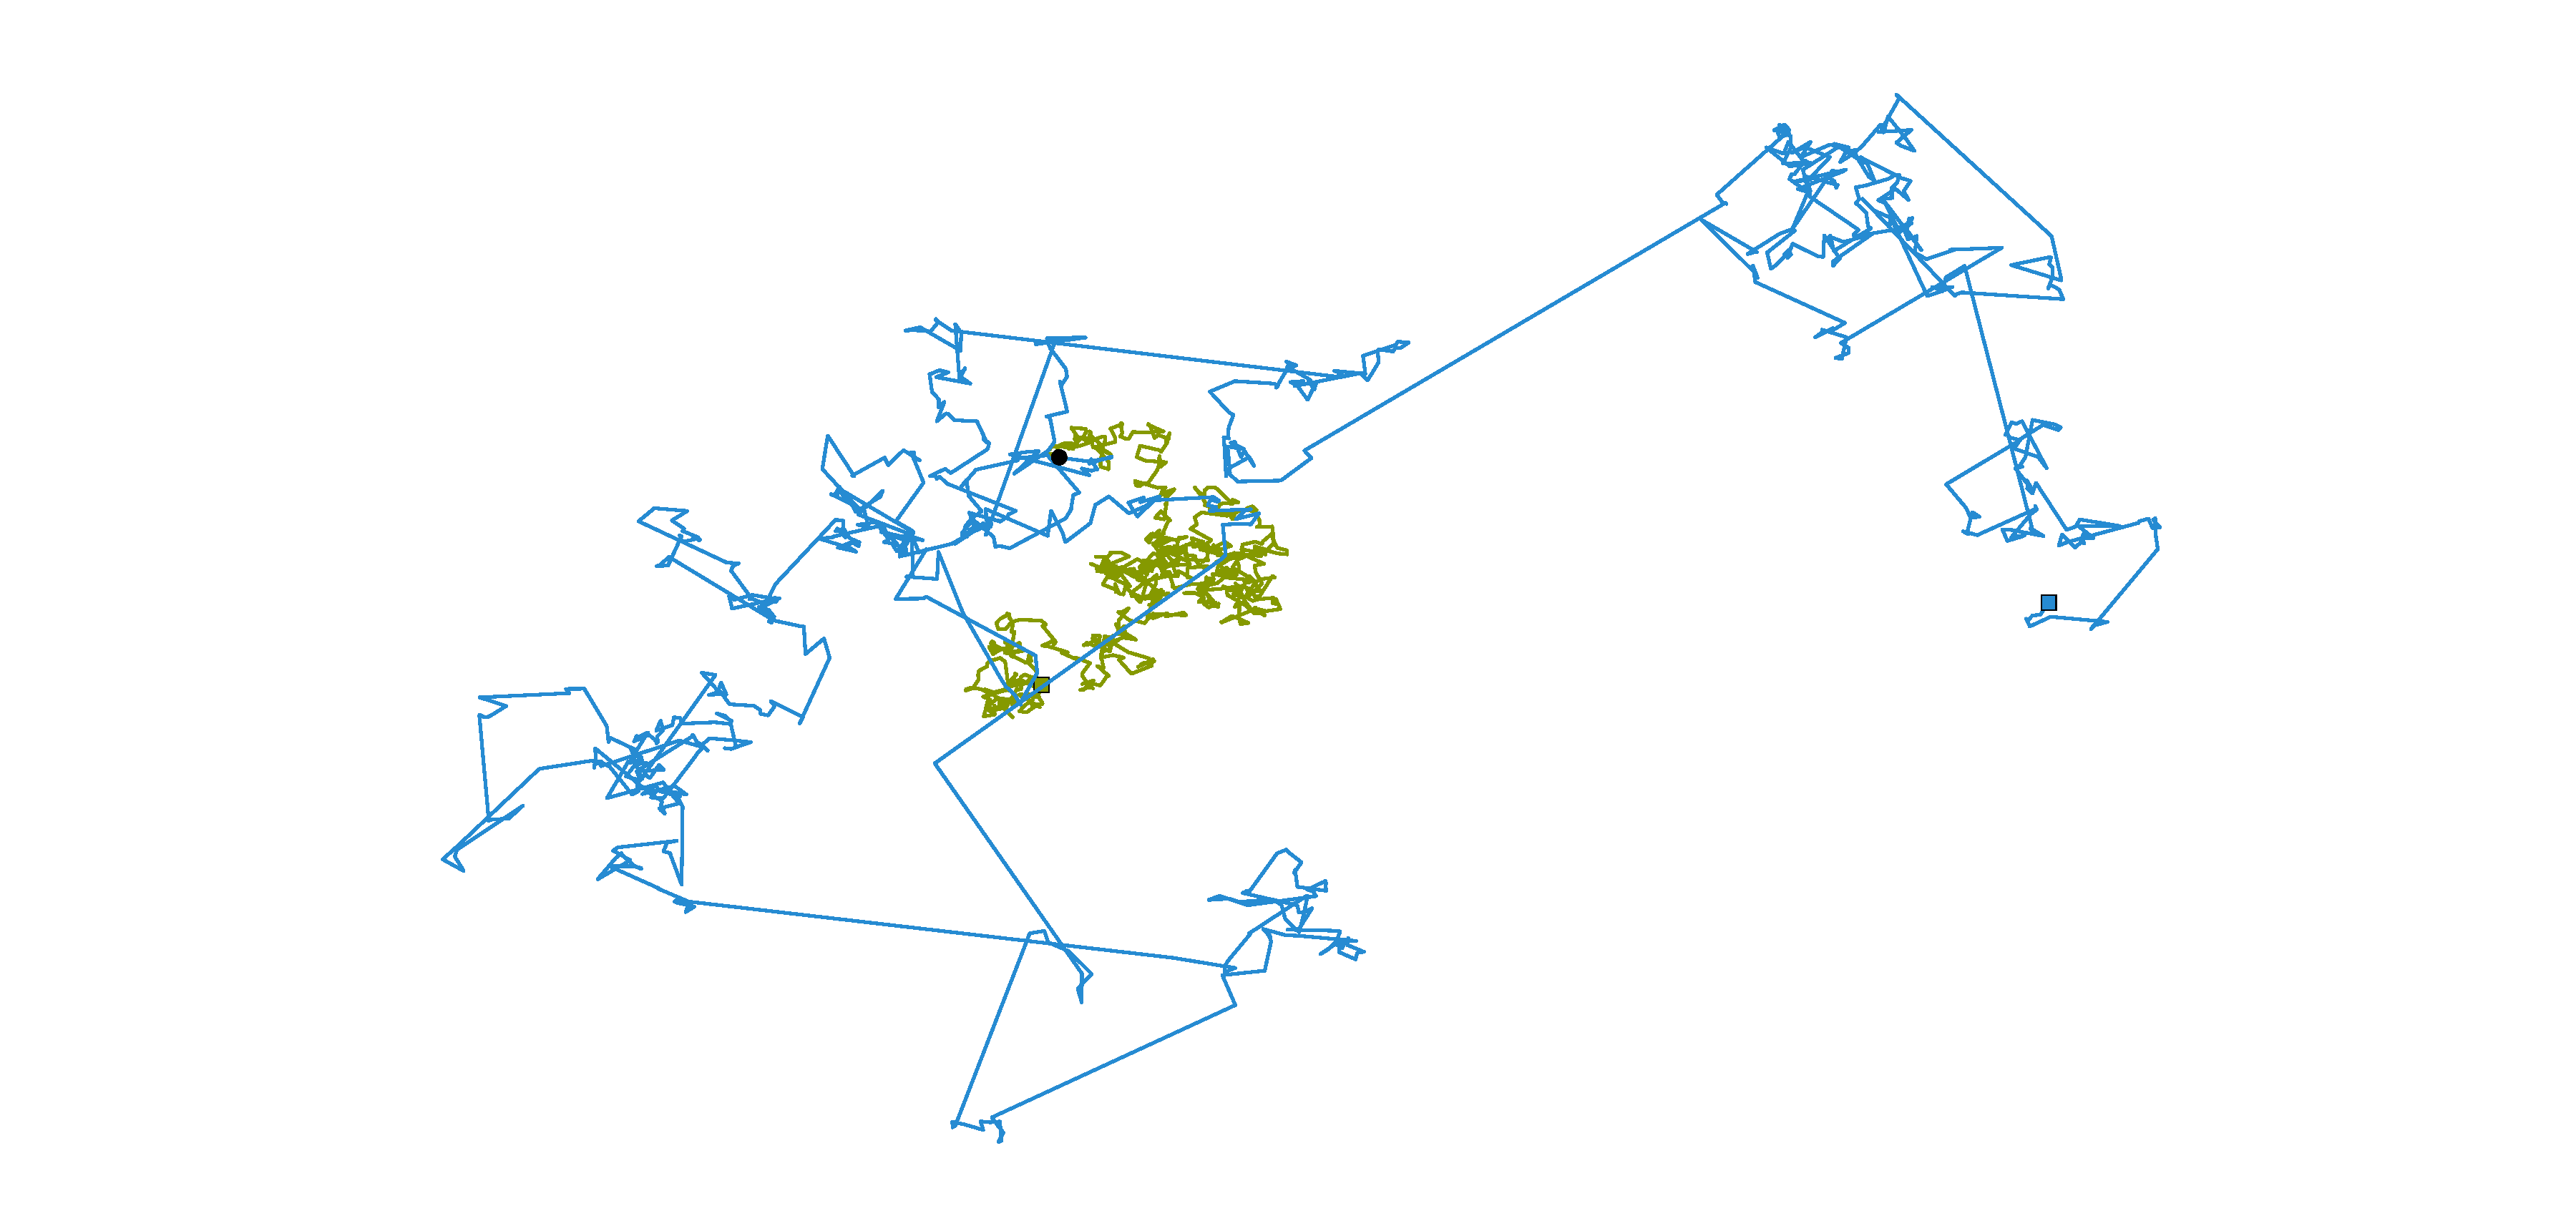
\includegraphics[width=0.6\textwidth, clip=True, trim=110mm 10mm 95mm 10mm]{Ressources/Images/Optimisation/LevyFlight/levy_vs_gaussian.pdf}
    \caption[Mouvement brownien et vol de \textit{Lévy} pour 200 pas aléatoires]
            {Mouvement brownien (en vert) et vol de \textit{Lévy} (en bleu) pour 200 pas aléatoires.}
    \label{fig:levy_vs_gaussian}
\end{figure}
% subsection vol_de_levy (end)


% ------------------------------------------------------------------------------
\subsection{Apprentissage par vecteur opposé} % (fold)
\label{sub:apprentissage_par_vecteur_oppose}
Les méthodes d’optimisation et spécifiquement les méthodes approchées sont fortement
dépendantes de la population initiale. Il est ainsi nécessaire
de constituer une population couvrant de manière homogène l’espace de décision.
L’approche la plus répandue consiste à construire une population initiale stochastiquement
à l’aide d’une distribution uniforme suivant \eqref{alg:init_phase}.
Afin d’améliorer la diversité / qualité de la population initiale sans connaissance
a priori, \textcite{Tizhoosh2005695} a développé l’apprentissage par vecteur opposé
(\abr{OBL} pour Opposite Based Learning) (\defref{def:oblm}).

\begin{Def}[OBL~:~Apprentissage par vecteur opposé]\label{def:oblm}
Admettons une position de dimension $D$, $\vec{x}(x_{1}, x_{2}, \dotsc, x_{D})$ avec
$x_{1}, x_{2}, \dotsc, x_{D}$ des valeurs bornées. Si $x_{j} \in [c_{j}, d_{j}]$ pour
$j = 1, 2, \dotsc, D$ alors la position opposée est $\vec{\check{x}}(\check{x_{1}},%
\check{x_{2}}, \dotsc, \check{x_{D}})$ est définie par:
\[\check{x_{j}} = c_{j} + d_{j} - x_{j}\]
\end{Def}

\textcite{Rahnamayan2008906} l’adaptent pour l’algorithme Differential Evolution (\abr{DE})
et montrent que la probabilité d’améliorer une solution est plus grande si on sélectionne
la position opposée que si on tire aléatoirement une autre position.
Dans leur implémentation, ils l’utilisent durant l’initialisation mais aussi au cours du
processus d’optimisation. Les bornes ($c_{j}$ et $d_{j}$) sont alors définies dynamiquement
afin d’éviter de ralentir la convergence.
Cette approche a aussi été appliquée avec succès dans le cas de l’algorithme \abr{ABC}
en association avec un opérateur de mutation \parencite{Bi2011174}, ou encore en coopération
avec une marche aléatoire \parencite{Sharma2012213}. Elle a aussi été utilisée pour
résoudre des problèmes à objectifs multiples, en combinaison avec un algorithme
évolutionnaire \parencite{Ma201448}, ou encore avec le \abr{PSO} \parencite{Gao2013114}.

L’approche est ainsi retenue afin d’améliorer la diversité de la population initiale
et sera aussi utilisée durant la phase des exploratrices afin d’augmenter la qualité
de la nouvelle position.
Pour chaque source, une position candidate ($\vec{x}$) et son opposée
($\vec{\check{x}}$) sont ainsi évaluées. Une sélection par tournoi binaire permet
de retenir la meilleure des deux comme nouvelle position pour la source.
% subsection apprentissage_par_vecteur_oppose (end)


\subsection[L’epsilon-dominance]{L’$\epsilon$-dominance} % (fold)
\label{sub:l_epsilon_dominance}
Contrairement à une approche mono-objectif, il existe plusieurs solutions optimales
dans une approche multi-objectifs. Il apparaît alors nécessaire de conserver l’évolution
du front de \textit{Pareto}~: c’est le rôle de l’archive \parencite{Laumanns2002263}.

Afin de garantir la convergence, il est nécessaire d’utiliser une approche élitiste
en limitant la population de l’archive aux solutions les plus performantes \parencite{Zitzler2000173}.
De plus, afin d’éviter de converger vers un front local, la population doit conserver
une bonne diversité.
L’algorithme de base du \abr{NSGA-II} \parencite{Deb2002182}, utilise le \textit{Fast
Non Dominated Sorting Algorithm} afin de construire son archive. Dans cette approche une
sélection par rang est appliquée afin de trier les solutions en différents niveaux et la
distance dite de crowding (distance moyenne entre deux solutions) est utilisée afin de
maintenir la diversité. L’algorithme \abr{SPEA II} améliore la diversité du
front final au prix d’une convergence plus lente en utilisant une approche par clustering.
Dans cette approche la taille limite de l’archive est définie par le nombre de clusters.
Ces clusters sont formés en se basant sur la distance euclidienne et une seule solution
est retenue.
\textcite{Laumanns2002263} proposent une autre approche, séparer l’espace des solutions en une
grille dont les dimensions sont définies par le vecteur $\vec{\epsilon}$. Dans cette
approche l’espace des objectifs est divisé en hypercubes, et chaque hypercube est comparé
selon l’$\epsilon$-dominance (\defref{def:eps_dominance}). Bien que d’autres
approches utilisent une grille similaire (\abr{PAES}) \parencite{Knowles2000149},
l’$\epsilon$-dominance n’accepte qu’une unique solution par hypercube assurant une plus
grande diversité de la population. La taille de l’archive est donc fonction des $\epsilon$
choisis pour chaque objectif et est donc toujours garantie d’être finie.


\begin{Def}[$\epsilon$-dominance]\label{def:eps_dominance}
L’$\epsilon$-dominance suppose que deux solutions sont identiques lorsqu’elles appartiennent
au même hypercube dont les dimensions des arêtes sont définies par
$\vec{\epsilon}_{m}, m \in \{1, \dotsc, M\}$ avec $M$ le nombre de fonctions objectif.
Dans le cas d’une maximisation il est dit que $\vec{x}_{a}$ $\epsilon$-domine $\vec{x}_{b}$ si~:
\begin{align*}
  \forall m \in \{1, M\}, \qquad
  \left\lceil\frac{f_{m}(\vec{x_{a}})}{\epsilon}\right\rceil &\leq
  \left\lceil\frac{f_{m}(\vec{x_{b}})}{\epsilon}\right\rceil  \\
  \intertext{et}
  \exists m \in \{1, M\}, \qquad
  \left\lceil\frac{f_{m}(\vec{x_{a}})}{\epsilon}\right\rceil &<
  \left\lceil\frac{f_{m}(\vec{x_{b}})}{\epsilon}\right\rceil  \\
\end{align*}
Cette relation sera notée~: $\vec{x}_{a} \prec_{\epsilon} \vec{x}_{b}$.
\end{Def}

Une solution peut ainsi être ou dominée, dominante, identique, ou non-dominée au sens de
l’$\epsilon$-dominance, les solutions $\epsilon$-non-dominées formant alors le front
d’$\epsilon$-Pareto (\figref{fig:epsilon_dominance}). Lors de l’ajout d’une solution à
l’archive l’$\epsilon$-dominance est dans un premier temps utilisée afin de les
départager. Dans le cas où la nouvelle solution serait $\epsilon$-identique elle est
uniquement comparée avec celle déjà archivée dans le même hypercube. La distance
euclidienne est alors utilisée pour les départager. La solution retenue est celle la plus
proche de l’optimum de l’hypercube (coin supérieur droit dans le cas d’une maximisation).
Contrairement à une sélection par dominance stricte le calcul de la distance euclidienne
permet de tenir compte de l’ensemble des amélioration et est moins élitiste. Afin d’éviter
l’ajout de biais, les objectifs sont normalisés dans l’espace de l’hypercube.
L’$\epsilon$-archive permet ainsi d’assurer~:
\begin{itemize}
  \item L’élitisme~: seule les solutions non-dominées sont retenues
  \item La diversification~: une unique solution par hypercube
  \item Une taille limite~: La taille maximale est fonction de $\vec{\epsilon}$ et est finie
  \item Une intensification~: En réduisant $\vec{\epsilon}$ on augmente la taille maximale de l’archive
  \item Une réduction~: En augmentant $\vec{\epsilon}$ on réduit la taille maximale de l’archive
\end{itemize}

\begin{figure}
    \centering
    \includegraphics[width=0.65\textwidth]{Ressources/Images/Optimisation/Epsilon_dominance/selection_boxes.pdf}
    \caption[Principe de la mise à jour de l’archive par epsilon-dominance]
            {Principe de la mise à jour de l’archive par epsilon-dominance (maximisation assumée).
             Adapté de \cite{Deb2005501}.}
    \label{fig:epsilon_dominance}
\end{figure}
L’étude réalisée par \textcite{Deb2005501} montre que l’$\epsilon$-dominance permet
d’obtenir une très bonne convergence et une grande diversité sur le front final.
Les résultats indiquent que les approches \abr{PESA} et \abr{NSGA II} obtiennent une moins
bonne représentation du front de Pareto que celles utilisant l’$\epsilon$-dominance
(\abr{$\epsilon$-MOEA}) ou le clustering (\abr{C-NSGA II}, \abr{SPEA}).
Cette observation est d’autant plus vraie pour des problèmes ayant plus de deux
objectifs (\textit{DTLZ1} \dots\ \textit{DTLZ7}).
De plus les résultats mettent aussi en évidence que le \abr{NSGA II} et le \abr{$\epsilon$-MOEA}
convergent plus rapidement que le \abr{SPEA II}.
Un désavantage à cette méthode peut cependant être noté. De par sa formulation
les solutions au niveau des extrêmes sur le front de Pareto sont plus difficilement
atteignables.

L’$\epsilon$-archive est donc retenue comme solution d’archivage dans ces travaux
car il représente un bon compromis entre diversité et convergence.
% subsection l_epsilon_dominance (end)


% ------------------------------------------------------------------------------
\subsection{Tenir compte des contraintes} % (fold)
\label{sub:tenir_compte_des_contraintes}
Les problèmes multi-objectifs dans le domaine de l’ingénierie sont souvent
dépendants de contraintes limitant l’ensemble des solutions optimales au domaine
de faisabilité. L’optimisation consiste alors à améliorer les objectifs tout en
respectant les contraintes spécifiques au problème \eqref{eq:def_optimisation}.

La littérature introduit de nombreuses méthodes permettant de tenir compte des
contraintes. L’approche la plus courante est d’utiliser un facteur de pénalité. Ce facteur
est dit statique si il est fixe durant l’ensemble de l’optimisation, dynamique si il est
adapté en fonction du nombre d’itérations, et adaptatif si les informations acquises par la
recherche aide à sa détermination \parencite{Coello2002}. Parmi les approches existantes il
peut être cité la méthode de la peine de mort. Elle consiste à appliquer une pénalité très
importante aux objectifs afin de rejeter toutes les solutions sous contraintes. Certaines
moins exclusives désavantagent les solutions ne respectant pas les contraintes en fonction
de leur niveau de violation alors que d’autres ajustent dynamiquement la pénalité en
fonction du nombre d’itérations déjà réalisées. Le problème récurrent avec ces approches
réside dans l’ajout de paramètres supplémentaires qui doivent être déterminés empiriquement.

\textcite{Coello2002} explique qu’une bonne prise en compte des contraintes ne devrait
pas nécessiter le paramétrage de facteurs car ils impactent
fortement la performance de la méthode. Finalement, la méthode sélectionnée ne
doit pas nécessiter un nombre plus important d’évaluations car elles peuvent être coûteuses.
\textcite{Deb2000311} propose une méthode de sélection par tournoi respectant ces conditions
dont les règles sont les suivantes~:
\begin{itemize}
  \item Une solution avec contraintes est inférieure à une solution sans contraintes
  \item Si les deux solutions sont sans contraintes la solution dominante est préférée
  \item Si les deux solutions sont sous contraintes, la solution violant le moins les contraintes est préférée
\end{itemize}
La méthode a l’avantage d’être simple à mettre en place mais est cependant
très élitiste car les solutions non faisables sont toujours écartées durant la
recherche.

Dans ces travaux la contrainte principale est l’obtention d’un bâtiment à énergie positive
favorisant le recours à l’énergie solaire par l’intermédiaire de capteurs photovoltaïques
et d’un \abr{SSC}. Cette contrainte limite fortement l’espace de recherche et une approche
trop stricte (qui considère toujours une solution sous contrainte comme inférieure) risque
de limiter l’exploratoire.
Dans ces travaux, une méthode adaptative moins élitiste est donc retenue. Adaptée
aux problèmes multi-objectifs par \textcite{Woldesenbet20073077}, la méthode ne demande
aucun paramétrage, et l’objectif modifié est calculé de la manière suivante~:
\begin{itemize}
  \item Normaliser les objectifs selon \eqref{eq:norm_obj}
  \item Normaliser les contraintes et les agréger pour former une unique contrainte selon \eqref{eq:norm_contrainte}
  \item Calculer les objectifs modifiés par agrégation des contraintes et des objectifs selon \eqref{eq:calc_modif_obj}
\end{itemize}

\begin{align}\label{eq:norm_obj}
  \tilde{f}_{m}(\vec{x}) &= \begin{cases}
    \frac{f_{m}(\vec{x}) - min(f_{m}(\vec{x}))}{max(f_{m}(\vec{x})) - min(f_{m}(\vec{x}))}
    & \text{(minimisation)} \\ \\ 1 - \left[\frac{f_{m}(\vec{x}) -
    min(f_{m}(\vec{x}))}{max(f_{m}(\vec{x})) - min(f_{m}(\vec{x}))}\right] &
    \text{(maximisation)} \\
  \end{cases}
\end{align}
avec $f_{m}(\vec{x})$ la valeur de l’objectif $m$, pour la position $\vec{x}$ dans l’espace de décision.

\begin{equation}\label{eq:norm_contrainte}
  v(\vec{x}) = \frac{1}{Q} \sum_{q=1}^{Q} \left(\frac{g_{q}(\vec{x})}{max(g_{q}(\vec{x}))}\right)
\end{equation}
avec $Q$ le nombre de contraintes d’inégalités. $g_{q}$ représente alors la fonction contrainte
associée à la contrainte $q$ avec $g_{q} \geq 0$. Dans cette représentation les contraintes
d’égalité doivent être transformées en contraintes d’inégalité.

\begin{equation}\label{eq:calc_modif_obj}
  F_{m}(\vec{x}) = d_{m}(\vec{x}) + p_{m}(\vec{x})
\end{equation}
avec $d_{m}(\vec{x})$ calculée selon \eqref{eq:dist_obj} et $ p_{m}(\vec{x})$ selon \eqref{eq:penalty_norm}.


\begin{align}\label{eq:dist_obj}
  d_{m}(\vec{x}) = \begin{cases}
                          v(\vec{x})                                     & \qquad si\  r_{f} = 0 \\
                          \sqrt{v(\vec{x})^2 + \tilde{f}_{m}(\vec{x})^2} & \qquad sinon          \\
                    \end{cases}
\end{align}
\begin{equation}\label{eq:penalty_norm}
  p_{m}(\vec{x}) = (1 - r_{f})  X(\vec{x}) + r_{f} Y_{m}(\vec{x})
\end{equation}

\begin{align*}
  \shortintertext{où} \\
    r_{f} &= \frac{\text{Nombre de solutions réalisables}}{\text{Taille de la population}} \\
  \shortintertext{et} \\
  X(\vec{x})     &= \begin{cases}
                0,          \qquad     & si\  r_{f} = 0\\
                v(\vec{x}), \qquad     & sinon\\
                \end{cases} \\
  Y_{m}(\vec{x}) &= \begin{cases}
                    0,          \quad \qquad & \text{si} \ \forall q, \ g_{q}(\vec{x}) = 0\\
                      \tilde{f}_{m}(\vec{x})  \\
            \end{cases}\\
\end{align*}

L’algorithme s’adapte ainsi dynamiquement à la population et peut accepter des
solutions ne respectant pas les contraintes. Plus il y a de solutions non
réalisables dans la population, moins une solution ne respectant pas les contraintes a
de chances d’être sélectionnée. L’approche permet d’améliorer l’exploration de
l’espace de décision et ainsi de pouvoir trouver des solutions existantes même
lorsque l’espace de faisabilité est faible.
L’approche est donc retenue dans ces travaux afin de mettre à jour la position des
sources, les solutions retenues dans l’archive doivent elles respecter
l’ensemble des contraintes pour être acceptées.
% subsection tenir_compte_des_contraintes (end)


% ------------------------------------------------------------------------------
\subsection{Description de l’approche globale} % (fold)
\label{sub:description_de_l_approche_globale}
Dans la section précédente, chaque élément utilisé dans l’algorithme a été détaillé et
les avantages et inconvénients des approches retenues ont aussi été explicités.
Dans cette section le fonctionnement global de la méthode approchée d’optimisation
multi-objectifs retenue est décrit.

L’algorithme (\figref{fig:abc_complet}) et le détail de chaque phase sont décrits ci-après.
Les sources sont initialisées (\algref{alg:init_phase}) suivant la méthode
\abr{OBL} (\defref{def:oblm}) afin d’obtenir une meilleure représentation du
domaine de décision en amont de l’optimisation.
Durant la phase des butineuses (\algref{alg:employed_phase}), chaque source
subit une variation en tenant compte de deux sources, une de l’essaim et une de l’archive.
Durant la phase des ouvrières (\algref{alg:onlooker_phase}), la qualité de
chaque source \eqref{eq:attribution_prob_to_source} est utilisée afin de sélectionner
et d’exploiter seulement les plus prometteuses. Finalement, si une source a été
modifiée infructueusement plus de $MaxEchec$, alors une exploratrice
réinitialise sa position de manière aléatoire  (\algref{alg:scout_phase}).
Tant que la condition d’arrêt n’est pas atteinte, les phases des butineuses,
des ouvrières, et des exploratrices sont répétées de manière cyclique. Au cours de
la recherche les nouvelles sources sont ajoutées à l’archive et sont utilisées
comme élément d’apprentissage pour les abeilles butineuses ou ouvrières. Les
exploratrices, elles, n’utilisent jamais d’éléments sociaux d’apprentissage.
Finalement, une fois la condition d’arrêt atteinte l’ensemble des solutions
de l’archive forme le front de Pareto.

\begin{figure}
    \centering
    \includegraphics[width=0.58\textwidth]{Ressources/Images/Optimisation/ABC/algorithme_complet.pdf}
    \caption[Description globale de l’algorithme ABC pour les problèmes multi-objectifs]
            {Description globale de l’algorithme ABC pour les problèmes multi-objectifs.}
    \label{fig:abc_complet}
\end{figure}

Dans l’optique de l’optimisation d’un modèle solaire développé sous \textit{Dymola}, l’algorithme
a été implémenté en \textit{Python} afin de faciliter le couplage avec la bibliothèque
\textit{DymTK} qui comme nous l’avons vu dans le chapitre précédent permet d’automatiser
la simulation concurrente de modèle \textit{Modelica} sous \textit{Dymola}. La bibliothèque est
disponible sous le nom de \textit{pyMayBee} et implémente~:
\begin{itemize}
  \item Une $\epsilon$-archive et la hypercube-dominance
  \item La dominance au sens de Pareto
  \item La prise en compte des contraintes suivant la méthode de \textcite{Woldesenbet20073077}
  \item Une interface commune permettant l’abstraction du type de variable (discrète, continue, qualitative)
  \item L’algorithme tel que décrit dans ces travaux
  \item Une suite de test unitaires et des cas théoriques validant l’approche avec
        et sans contraintes
\end{itemize}

L’approche retenue contrairement à la majorité des méta-heuristiques demande
peu de paramètres à définir de manière empirique et est ainsi robuste. En effet
seule la taille de la population $NP$, et le nombre d’essais maximum $MaxEchec$ sont à définir.
De plus la taille de la population n’impacte pas le nombre de solutions dans l’archive
car le stockage est réalisé dans une structure indépendante. Il est aussi important
de noter que les deux uniques paramètres ont un comportement prévisible facilitant
leur paramétrage. La taille de la population en augmentant améliore l’exploration
réduisant les risques de stagner vers des optimums locaux mais réduit la vitesse
de convergence (\defref{def:convergence}).
Le nombre d’essais maximum lui est directement lié au nombre de variables de décision
et à la taille de la population. Une valeur faible se traduit par un abandon rapide
des solutions alors qu’une valeur plus grande augmente le nombre de variations évaluées
pour chaque source. Ainsi on note clairement l’impact de chaque paramètre sur la
performance de l’algorithme simplifiant sa paramétrisation.

% Add algorithmes
%!TEX root = ../main.tex
% Algorithme/pyMayBee.tex

% Comments
\newcommand\commfont[1]{\footnotesize\ttfamily\textcolor{SolarizedBrCyan}{#1}}
\SetCommentSty{commfont}
\SetKwComment{AComment}{\#~}{}

% Functions
\SetKwFunction{ALevyFlight}{LevyFlight}
\SetKwFunction{ALevy}{Levy}

% Keywords
\SetKwData{ASources}{Sources}
\SetKwData{ASource}{Source}
\SetKwData{AButineuse}{Butineuse}
\SetKwData{AOuvriere}{Ouvrière}
\SetKwData{ANbrSources}{N}
\SetKwData{AOnlookers}{Ouvrières}
\SetKwData{AScouts}{Éclaireuses}
\SetKwData{AEmployed}{Butineuses}
\SetKwData{ABee}{Abeille}
\SetKwData{ABees}{Abeilles}
\SetKwData{AHive}{Essaim}
\SetKwData{AVariables}{Variables}
\SetKwData{AVariable}{Variable}
\SetKwData{ANbrVariables}{J}
\SetKwData{AArchive}{Archive}
\SetKwData{APopulation}{Population}
\SetKwData{ATirageA}{TirageA}
\SetKwData{ATirageB}{TirageB}
\SetKwData{ARatio}{Ratio}
\SetKwData{AMR}{MR}
\SetKwData{ATrial}{échec}
\SetKwData{AMaxTrial}{$Max_{échec}$}


% Phase d’initialisation
\begin{algorithm}[!htb]
  \SetAlgoVlined
  \DontPrintSemicolon
  \emph{Initialisation des \ASources sur l’ensemble de l’espace de décision}\;
  \For{$i \leftarrow 0$ \KwTo \ANbrSources}
  {
    \emph{Initialisation des variables de décision pour chaque source}\;
    \For{$j \leftarrow 0$ \KwTo \ANbrVariables}
    {
      \circled[b]{a} \emph{Initialisation de la position de la $\ASource_{i}$ de manière aléatoire}\;
      \Indp
      $x_{ij} = x_{j}^{min} + RandUniform(0, 1) \times (x_{j}^{max} - x_{j}^{min})$\;
      \Indm
      \BlankLine
      \circled[b]{b}  \emph{Génération de l’$\ABee_{i}$ dont la position est calculée suivant Définition~\ref{def:oblm}}\;
      \Indp
      $ \check{x_{ij}} = x_{j}^{min} + x_{j}^{max} - x_{ij}$\;
      \Indm
      \BlankLine
      \circled[b]{c} \emph{Évaluation de la $\ASource_{i}$ et de l’$\ABee_{i}$}\;
      \BlankLine
      avec $RandUniform$ un tirage aléatoire suivant une loi uniforme, et $x_{j}^{min}$, $x_{j}^{max}$
      respectivement le minimum et le maximum de la variable $j$\;
    }
    \If{$\ASource_{i}$ respecte toutes les contraintes}
    {
      $\AArchive \pluseq \ASource_{i}$ \AComment{On ajoute la source initial à l’archive}
    }
    \If{$\ABee_{i}$ respecte toutes les contraintes}
    {
      $\AArchive \pluseq \ABee_{i}$ \AComment{On ajoute la source opposée à l’archive}
    }
  }
  Mise à jour des \ASources d’après Algorithm~\ref{alg:maj_phase}\;
  \caption[Initialisation des sources par \abr{OBLM}]
          {Initialisation des sources par \abr{OBLM} (Définition~\ref{def:oblm}).}
  \label{alg:init_phase}
\end{algorithm}


% Phase des éclaireuses
\begin{algorithm}[!htb]
  \SetAlgoVlined
  \DontPrintSemicolon
  \AComment{Exploration par les \AScouts}
  \For{$i \leftarrow 0$ \KwTo \ANbrSources}
  {
    \If{$\ATrial_{i} > \AMaxTrial$ }
    {
      Génération de deux nouvelles positions suivant Algorithm~\ref{alg:init_phase}\;
    }
  }
  Mise à jour de la position des \ASources d’après Algorithm~\ref{alg:maj_phase}\;
  \caption[Phase des éclaireuses]
          {Phase des éclaireuses.}
  \label{alg:scout_phase}
\end{algorithm}


% Phase des ouvrières
\begin{algorithm}[!htb]
  \SetAlgoVlined
  \DontPrintSemicolon
  \AComment{Exploitation des sources par les \AOnlookers}
  \AComment{Plusieurs \AOnlookers peuvent modifier la même source}
  \For{$\AOuvriere \in \AOnlookers$}
    {
      Sélection aléatoire d’une \ASource $i$ selon la probabilité
      définie par l’équation \eqref{eq:attribution_prob_to_source}\;
      Sélection aléatoire d’une source $a$ ($a \neq i$) dans l’\AArchive\;
      \circled[b]{a} \emph{Génération d’une nouvelle position $\vec{x_{i}}'$ à partir de la
                         position $\vec{x_{i}}$ pour l’\AOuvriere }\;
      \For{$j \leftarrow 0$ \KwTo \ANbrVariables}
      {
      \begin{algomathdisplay}
        x_{ij}' =%
          \begin{cases}
            x_{ij}  + RandUniform(-1, 1)   \times \ (x_{ij} - x_{aj}) &\ \ATirageB < \AMR \\
            x_{ij}                                                    &\ sinon
          \end{cases}
      \end{algomathdisplay}
      }
      \BlankLine
      Avec \AMR est la probabilité de réaliser une modification (fixée à \num{0.2}) et
      \ATirageB un nombre aléatoire entre \num{0} et \num{1}\;
      \BlankLine
      \circled[b]{b} \emph{Évaluation des objectifs pour la nouvelle position $\vec{x_{i}}'$}\;
      \BlankLine
      \If{\AOuvriere respecte toutes les contraintes}
      {
        $\AArchive \pluseq \AOuvriere$ \AComment{Ajout de la solution trouvée par l’\AOuvriere à l’archive}
      }
    }

  Mise à jour de la position des \ASources qui ont été modifiées d’après Algorithme~\ref{alg:maj_phase}\;
  \caption[Phase des ouvrières]
          {Phase des ouvrières.}
  \label{alg:onlooker_phase}
\end{algorithm}


% Maj des sources
\begin{algorithm}[!htb]
  \SetAlgoVlined
  \DontPrintSemicolon
  Récupérer le maximum et minimum pour chaque objectif et contraintes dans l’\AHive\;
  \For{$\ABee \in \ABees$}
  {
    Calcul du vecteur objectif pour l’\ABee ($\vec{F}'_{i}$) et pour sa \ASource $i$ ($\vec{F}_{i}$),
    respectivement aux positions $\vec{x_{i}}'$ et $\vec{x_{i}}$
    selon \eqref{eq:calc_modif_obj}\;
    \For{$m \leftarrow 1$ \KwTo M}
    {
      \begin{algomathdisplay}
      \begin{aligned}
      F_{im}' &= d_{m}'(\vec{x_{i}}) + p_{m}'(\vec{x_{i}}) \\
      F_{im}  &= d_{m}(\vec{x_{i}}) + p_{m}(\vec{x_{i}})   \\
      \end{aligned}
      \end{algomathdisplay}
    }
    \If{$\vec{x_{i}}' \succ \vec{x_{i}}$}
    {

      $\ASource_{i} \leftarrow \ABee$ \AComment{Mise à jour de la \ASource à partir de l’\ABee}

      $\ATrial_{i} \leftarrow 0$ \AComment{On réinitialise le nombre d’essais pour la \ASource $i$}
    }
    \Else
    {
      $\ATrial_{i} \pluseq 1$ \AComment{On incrémente le nombre d’essais pour la \ASource $i$}
    }
  }
  \caption[Mise à jour des Sources par les Abeilles]
          {Mise à jour des \textbf{Sources} par les \textbf{Abeilles}.}
  \label{alg:maj_phase}
\end{algorithm}


% Phase des butineuses
\begin{algorithm}[!htb]
  \SetAlgoVlined
  \DontPrintSemicolon
  \AComment{Exploration des sources par les \AEmployed}
  \For{$i \leftarrow 0$ \KwTo \ANbrSources}
  {
    Sélection aléatoire de $2$ sources~: $a$ ($a \neq i$) dans l’\AArchive, et $b$ ($b \neq i$) dans l’\AHive\;
    \BlankLine
    \circled[b]{a} \emph{Génération d’une nouvelle position $\vec{x_{i}}'$ à partir de la %
                       position $\vec{x_{i}}$ pour la \AButineuse $i$}\;
    \If{$\ATirageA < \ARatio $ }
      {
      \For{$j \leftarrow 0$ \KwTo \ANbrVariables}
      {
      \begin{algomathdisplay}
        x_{ij}' =%
          \begin{cases}
            \begin{aligned}
              x_{ij}  &+ \num{0.01} \times ~\ALevy  &\times (x_{ij} - x_{bj})  \\
                      &+ \num{0.01} \times |\ALevy|   &\times (x_{aj} - x_{ij})  \\
            \end{aligned} &\ \ATirageB < \AMR \\
            x_{ij}        &\ sinon
          \end{cases}
      \end{algomathdisplay}
      \ALevy est nombre aléatoire dans une distribution de Lévy (Définition~\ref{def:vol_levy})\;
      }
      }
    \Else
      {
      \For{$j \leftarrow 0$ \KwTo \ANbrVariables}
      {
      \begin{algomathdisplay}
        x_{ij}' =%
          \begin{cases}
            \begin{aligned}
              x_{ij}  &+ RandUniform(-1, 1)   &\times \ (x_{ij} - x_{bj})  \\
                      &+ RandUniform(0, 1)    &\times \ (x_{aj} - x_{ij})  \\
            \end{aligned} &\ \ATirageB < \AMR \\
            x_{ij}        &\ sinon
          \end{cases}
      \end{algomathdisplay}
      }
      }
      Où \ARatio est la probabilité de réaliser un vol de Lévy (fixée à \num{0.5}), et \AMR la probabilité
      de réaliser une modification (fixée à \num{0.3}). \ATirageA et \ATirageB étant des nombres aléatoires
      (entre \num{0} et \num{1}) tirés dans une distribution uniforme\;
      \BlankLine
    \circled[b]{b} \emph{Évaluation des objectifs pour la nouvelle position $\vec{x_{i}}'$}\;
    \If{$\AButineuse_{i}$ respecte toutes les contraintes}
    {
      \AComment{On ajoute la nouvelle source à l’archive}
      $\AArchive \pluseq \AButineuse_{i}$\;
    }
  }
%   \AComment{On ne conserve qu’une seule position par source}
  Mise à jour de la position des \ASources d’après Algorithme~\ref{alg:maj_phase}\;
  \caption[Phase des butineuses]{Phase des butineuses.}
  \label{alg:employed_phase}
\end{algorithm}


% subsection description_de_l_approche_globale (end)


% ------------------------------------------------------------------------------
\subsection{Validation de la méthode} % (fold)
\label{sub:validation_de_la_methode}
Cette section permet d’apprécier la performance de l’approche pour différents types
de problèmes pouvant être rencontrés dans un problème d’optimisation.

La bibliothèque \textit{pyMayBee} a été développée autour de tests unitaires (\enquote
{Test-driven development}). Chaque élément (fonction / méthodes /\dots) et comportement
(minimisation / maximisation /\dots) a ainsi été testé afin de garantir que la
bibliothèque implémente correctement les éléments et comportements nécessaires. De par
son approche, chaque nouvelle modification tient implicitement compte des tests précédents
et garanti ainsi l’intégrité du code lors de son développement. Après l’implémentation
des briques nécessaires et la construction de l’algorithme, des problèmes étalons ont été
utilisés afin de valider la performance de l’approche. Bien que la réussite d’un problème
étalon ne soit pas une condition suffisante pour garantir la convergence sur un problème
réel, il apporte une information importante~: la capacité de l’algorithme à s’adapter aux
différents types de contraintes pouvant survenir.

La littérature décrit déjà les bénéfices apportée par l’utilisation du vol de
\textit{Lévy}, de l’\abr{OBL}, de l’$\epsilon$-dominance, ou encore de la prise en compte
dynamique des contraintes. Ainsi, cette section n’a pas vocation a montrer le bénéfice
apporté par les différentes améliorations proposées. Il reste cependant nécessaire de
montrer que l’implémentation de l’algorithme \abr{ABC} fonctionne correctement. Dans cette
optique les résultats présentés dans cette section sont sélectionnés afin de couvrir les
principales difficultés existantes \parencite{Collette2002,Deb2002825}~:
\begin{itemize}
    \item Front linéaire~: \textit{Hanne1} et \textit{DTLZ1}
    \item Front convexe~: \textit{ZDT1}
    % \item Front concave~: \textit{ZDT2}
    \item Multi-modal~: \textit{ZDT4}
    \item Concave + non-uniformité avec faible densité près de l’optimal~: \textit{ZDT6} et \textit{DTLZ5}
    \item Discontinue~: \textit{DTLZ7}
\end{itemize}

Les résultats obtenus sont comparés aux résultats obtenus par \textcite{Deb2005501}
pour différents algorithmes couramment utilisés à travers l’hypervolume et la
distance générationnelle (\tabref{tab:evaluation_algo_opti}). Une augmentation de l’hypervolume
se traduit par une meilleure convergence et couverture de l’espace des objectifs par l’ensemble des solutions.
À l’inverse plus la distance générationnelle est faible, plus l’approximation obtenue par l’algorithme
est proche du vrai front de \textit{Pareto}~: l’indicateur traduit la qualité de convergence.
Comme pour les algorithmes de l’article, on considère \num{20000} évaluations pour les problèmes avec deux
objectifs et \num{30000} évaluations pour les problèmes avec trois objectifs.
Les résultats montrent que l’algorithme permet d’obtenir une bonne convergence et une bonne
répartition des solutions sur le front de Pareto. Il obtient de plus un écart type très bas
que ce soit sur l’hypervolume ou sur la distance générationnelle traduisant la robustesse de
l’approche. Il n’est pas le plus performant en moyenne, cependant il est toujours proche de l’algorithme le plus
performant contrairement aux algorithmes \textit{PESA}, \textit{$\epsilon$-MOEA}, et \textit{NSGAII} dont les
résultats pour le problème \textit{ZDT6} sont loin des valeurs obtenues par \textit{SPEA $2$} et
\textit{pyMayBee}.
Les indicateurs pour les problèmes \textit{DTLZ1} et \textit{DTLZ7} sont aussi
présentés graphiquement afin d’apprécier la convergence et l’étendue de la répartition du front
(\figref{fig:convergence_pareto_pymaybee}). Le front du problème \textit{DTLZ1} met
clairement en évidence l’uniformité des solutions grâce à l’$\epsilon$-archive et la
convergence sur le problème \textit{DTLZ7}, sa capacité à trouver des solutions pour des fronts discrets.

L’algorithme d’optimisation multi-objectifs décrit dans ce chapitre permet donc
d’obtenir une bonne convergence et une bonne répartition pour une large variété de problèmes.
Il est donc utilisé dans le chapitre suivant pour réaliser l’étude de cas.

\begin{table}
\centering
\caption[Évaluation des solutions des fronts de Pareto obtenues à partir de différents algorithmes]
        {Comparaison de la qualité de convergence et de la qualité de répartition des
         solutions des fronts de Pareto obtenues à partir de différents algorithmes.}
\label{tab:evaluation_algo_opti}
\begin{tabular}{L{4cm} c c c c c}
  \toprule
  \addlinespace
                           & \multicolumn{2}{c}{\textbf{Distance générationnelle}} & & \multicolumn{2}{c}{\textbf{Hypervolume}} \\
                           & Moyenne     & Écart type                 & & Moyenne & Écart type                                  \\
  \addlinespace[\defaultaddspace]
  \multicolumn{6}{l}{\textbf{Hanne1} ($2$ objectifs)}                                                                     \\
  \midrule
  \textit{pyMayBee}        & \num{5.036E-02} & \num{2.343E-03} & & \num{13.1691} & \num{0.01743428} \\
  \\
  \addlinespace[\defaultaddspace]
  \multicolumn{6}{l}{\textbf{\abr{ZDT1}} ($2$ objectifs)}                                                                          \\
  \midrule
  \textit{PESA}            & \num{5.348E-04} & \num{1.262E-04} & & \num{0.8680} & \num{6.76E-04} \\
  \textit{NSGAII}          & \num{5.490E-04} & \num{6.620E-05} & & \num{0.8701} & \num{3.85E-04} \\
  \textit{SPEA2}           & \cellcolor{SolarizedBrWhite} \num{1.006E-03} & \num{1.206E-04} & & \cellcolor{SolarizedBrWhite} \num{0.8708} & \num{1.86E-04} \\
  \textit{$\epsilon$-MOEA} & \num{3.955E-04} & \num{1.220E-05} & & \num{0.8702} & \cellcolor{SolarizedBrWhite} \num{8.25E-05} \\
  \textit{pyMayBee}        & \num{3.662E-04} & \cellcolor{SolarizedBrWhite} \num{2.510E-05} & & \num{0.8696} & \num{2.74E-04} \\
  \\
  % \addlinespace[\defaultaddspace]
  % \multicolumn{6}{l}{\textbf{\abr{ZDT2}} ($2$ objectifs)}                                                                              \\
  % \midrule
  % \textit{PESA}            & \num{3.794E-04} & \num{2.950E-05} & & \num{0.5329}  & \num{1.13E-03} \\
  % \textit{NSGAII}          & \cellcolor{SolarizedBrWhite} \num{3.785E-04} & \cellcolor{SolarizedBrWhite} \num{1.880E-05} & & \num{0.5372}  & \num{3.01E-04} \\
  % \textit{SPEA2}           & \num{8.285E-04} & \num{1.138E-04} & & \num{0.5374}  & \num{2.61E-04} \\
  % \textit{$\epsilon$-MOEA} & \num{4.645E-04} & \num{2.470E-05} & & \cellcolor{SolarizedBrWhite} \num{0.5383}  & \cellcolor{SolarizedBrWhite} \num{6.39E-05} \\
  % \textit{pyMayBee}        & \num{4.468E-04} & \num{4.149E-05} & & \num{0.5281}  & \num{1.20E-04} \\
  % \\
  \addlinespace[\defaultaddspace]
  \multicolumn{6}{l}{\textbf{\abr{ZDT4}} ($2$ objectifs)}                                                                              \\
  \midrule
  \textit{PESA}            & \num{7.302E-03} & \num{4.700E-03} & & \num{0.8566} & \num{6.40E-03} \\
  \textit{NSGAII}          & \num{6.390E-03} & \num{4.300E-03} & & \cellcolor{SolarizedBrWhite} \num{0.8613} & \num{7.10E-03} \\
  \textit{SPEA2}           & \num{7.693E-03} & \num{4.300E-03} & & \num{0.8609} & \num{5.36E-03} \\
  \textit{$\epsilon$-MOEA} & \cellcolor{SolarizedBrWhite} \num{2.591E-03} & \num{6.000E-04} & & \num{0.8509} & \num{1.54E-02} \\
  \textit{pyMayBee}        & \num{3.408E-03} & \cellcolor{SolarizedBrWhite} \num{2.205E-04} & & \num{0.8580} & \cellcolor{SolarizedBrWhite} \num{4.59E-03} \\
  \\
  \addlinespace[\defaultaddspace]
  \multicolumn{6}{l}{\textbf{\abr{ZDT6}} ($2$ objectifs)}                                                                              \\
  \midrule
  \textit{PESA}            & \num{6.416E-02} & \num{7.300E-03} & & \num{0.4145} & \num{9.90E-03} \\
  \textit{NSGAII}          & \num{7.896E-02} & \num{6.700E-03} & & \num{0.3959} & \num{8.94E-03} \\
  \textit{SPEA2}           & \cellcolor{SolarizedBrWhite} \num{5.736E-03} & \num{9.000E-04} & & \cellcolor{SolarizedBrWhite} \num{0.4968} & \num{1.17E-03} \\
  \textit{$\epsilon$-MOEA} & \num{6.793E-02} & \num{1.180E-02} & & \num{0.4112} & \num{1.57E-02} \\
  \textit{pyMayBee}        & \num{1.770E-02} & \cellcolor{SolarizedBrWhite} \num{2.518E-04} & & \num{0.4957} & \cellcolor{SolarizedBrWhite} \num{5.91E-05} \\
  \\
  \addlinespace[\defaultaddspace]
  \multicolumn{6}{l}{\textbf{\abr{DTLZ1}} ($3$ objectifs)}                                                                              \\
  \midrule
  \textit{PESA}            & \num{3.600E-03} & \num{2.900E-03} & & \num{0.2825} & \num{3.32E-03} \\
  \textit{NSGAII}          & \num{3.510E-03} & \cellcolor{SolarizedBrWhite} \num{6.700E-04} & & \num{0.3132} & \num{5.89E-04} \\
  \textit{SPEA2}           & \num{3.330E-03} & \num{3.541E-02} & & \cellcolor{SolarizedBrWhite} \num{0.3160} & \cellcolor{SolarizedBrWhite} \num{6.98E-04} \\
  \textit{$\epsilon$-MOEA} & \cellcolor{SolarizedBrWhite} \num{3.290E-03} & \num{9.200E-04} & & \num{0.3009} & \num{1.50E-03} \\
  \textit{pyMayBee}        & \num{4.700E-03} & \num{2.464E-03} & & \num{0.3006} & \num{1.03E-03} \\
  \\
  \addlinespace[\defaultaddspace]
  \multicolumn{6}{l}{\textbf{\abr{DTLZ5}} ($3$ objectifs)}                                                                          \\
  \midrule
  \textit{PESA}            & \num{9.463E-04} & \num{1.143E-04} & & &                \\
  \textit{NSGAII}          & \num{2.083E-03} & \num{1.198E-04} & & &                \\
  \textit{SPEA2}           & \num{1.978E-03} & \num{1.644E-04} & & &                \\
  \textit{$\epsilon$-MOEA} & \cellcolor{SolarizedBrWhite} \num{9.536E-04} & \num{4.892E-05} & & &                \\
  \textit{pyMayBee}        & \num{1.598E-03} & \cellcolor{SolarizedBrWhite} \num{4.741E-05} & & \num{0.4292} & \num{9.57E-06}  \\
  \\
  \addlinespace[\defaultaddspace]
  \multicolumn{6}{l}{\textbf{DTL7} ($3$ objectifs)}                                                                       \\
  \midrule
  \textit{pyMayBee}        & \num{1.990E-02} & \num{6.880E-04} & & \num{1.2346} & \num{9.89E-03} \\
  \bottomrule
  \end{tabular}
\end{table}

\begin{figure}
    \centering
    \begin{subfigure}[b]{0.49\textwidth}
        \centering
        \includegraphics[width=\textwidth, clip=True, trim=50mm 10mm 50mm 10mm]{Ressources/Images/Optimisation/Validation/dtlz1.pdf}
        \caption{}
        \label{fig:dtlz1}
    \end{subfigure}
    \begin{subfigure}[b]{0.49\textwidth}
        \centering
        \includegraphics[width=\textwidth, clip=True, trim=50mm 10mm 50mm 10mm]{Ressources/Images/Optimisation/Validation/dtlz7.pdf}
        \caption{}
        \label{fig:dtlz7}
    \end{subfigure}
    \quad
    \caption[Front de \textit{Pareto} obtenu pour trois problèmes distincts]
             {Comparaison entre le front de \textit{Pareto} obtenu grâce à la bibliothèque
              \textit{pyMayBee} et le vrai front de \textit{Pareto} pour les
              problèmes \textit{DTLZ1} (a) et \textit{DTLZ7} (b).}
    \label{fig:convergence_pareto_pymaybee}
\end{figure}
% subsection validation_de_la_methode (end)
% section algorithme_de_colonie_d_abeilles_virtuelles (end)


\section{Bilan} % (fold)
\label{sec:bilan_methodologie}
Au cours de ce chapitre une méthodologie d’aide à la décision permettant d’accompagner les
concepteurs pour le dimensionnement d’un \abr{SSC} couplé à une \abr{MEPOS} a été
développée. La complexité du modèle est limitée grâce à une analyse
de sensibilité globale puis le temps d’évaluation du modèle est réduit en utilisant des
méta-modèles. Bien que nécessaire dans ce cas précis, il reste préférable de conserver le
modèle original dans le cas où il peut être évalué dans un temps raisonnable afin d’éviter
d’introduire une erreur d’approximation. Pour l’aide à la décision, une approche a
posteriori par coordonnées parallèles est retenue afin de ne pas introduire de préférences
en amont et permettre d’explorer de nouvelles combinaisons. Cette approche
nécessite l’obtention préalable d’un ensemble de solutions non-dominées et le choix d’une
méthode d’optimisation multi-objectifs est donc nécessaire. Le problème étant fortement
combinatoire, une méta-heuristique s’est imposé comme le choix le plus adapté. Afin de
proposer une approche à la fois simple, intuitive et performante, un algorithme de colonie
d’abeilles virtuelles (\abr{ABC}) a été adaptée aux problèmes multi-objectifs. Ce choix a
été retenu principalement car l’approche ne nécessite le paramétrage que de trois
paramètres dont l’impact est connu a priori. L’approche a ensuite été renforcée par
l’ajout d’une archive garantissant une bonne diversité de la population, et d’un vol de
Lévy pour éviter la stagnation et améliorer l’exploratoire. De plus, durant
l’initialisation, le choix a été fait de retenir l’\abr{OBLM} (\defref{def:oblm}) afin
d’offrir une meilleure répartition des solutions. Finalement, afin d’améliorer
l’exploration et l’exploitation de l’espace de faisabilité, les contraintes
sont prises en compte dynamiquement. Contrairement à une approche statique et stricte plus
classique, des solutions non faisables peuvent être conservées apportant ainsi de nouvelles
connaissances sur le problème. Il est ensuite possible par apprentissage, d’obtenir de
nouvelles solutions optimales même dans un domaine fortement contraint.

La \figref{fig:outils_methode} récapitule l’ensemble des outils utilisés pour la
mise en place de la méthodologie. Comme pour l’étude
paramétrique, les bibliothèques \textit{Buildingspy} et \textit{DymTK} sont utilisées
afin de pouvoir automatiser la simulation en parallèle des modèles à partir du langage
\textit{Python}. \textit{DyMat} a permis quant à elle de lire les résultats qui sont
ensuite traités grâce aux bibliothèques \textit{Pandas} et \textit{Numpy}. Afin de réaliser
l’échantillon pour le criblage de \textit{Morris}, la bibliothèque \textit{Salib} est retenue.
Pour la construction d’un échantillon uniformément réparti par méthode de Quasi-Monte-Carlo
et la création des méta-modèles, la bibliothèque \textit{OpenTurns} est utilisée.
L’optimisation est réalisée par une méta-heuristique et implémentée dans la bibliothèque \textit{pyMayBee}.
Finalement l’aide à la décision est réalisée par une méthode de coordonnées
parallèles grâce au logiciel \textit{XDAT}.
La mise en place de cette méthodologie est illustrée dans le dernier chapitre à travers l’étude
de la performance du \abr{SSC} sur Bordeaux et Strasbourg.

\begin{figure}
    \centering
    \includegraphics[width=0.9\textwidth]{Ressources/Images/chapitre3_bilan.pdf}
    \caption[Outils utilisés pour la mise en place de la méthodologie d’aide à la décision]
            {Outils utilisés pour la mise en place de la méthodologie d’aide à la décision.}
    \label{fig:outils_methode}
\end{figure}

% section bilan_methodologie (end)
